\documentclass[11pt,a4paper]{article}
\newcommand{\gls}[1]{#1\textsubscript{G}}
\usepackage[utf8]{inputenc}
\usepackage[italian]{babel}
\usepackage{geometry}
\usepackage{graphicx}
\usepackage{float}
\usepackage{tabularx}
\usepackage{booktabs}
\usepackage{hyperref}
\usepackage{fancyhdr}
\usepackage{lastpage}
\usepackage{longtable}

\geometry{margin=2.5cm}

% Intestazione e piè di pagina
\pagestyle{fancy}
\fancyhf{}
\renewcommand{\headrulewidth}{0pt}
\fancyfoot[C]{\thepage\ di \pageref{LastPage}}

\begin{document}

% Prima pagina - Intestazione
\begin{titlepage}
    \centering
    
    % Logo Università
    \begin{figure}[H]
        \centering
        
\includegraphics[width=0.3\textwidth]{../logoUnipd.jpg}
    \end{figure}
    
    \vspace{0.5cm}
    
    \textbf{\Large Università degli Studi di Padova} \\
    \vspace{0.2cm}
    \textbf{Laurea in Informatica} \\
    \vspace{0.2cm}
    \textbf{Corso di Ingegneria del Software} \\
    \vspace{0.2cm}
    \textbf{Anno Accademico 2025/2026} \\
    
    \vspace{1cm}
    
    % Logo gruppo
    \begin{figure}[H]
        \centering
        
\includegraphics[width=0.2\textwidth]{../LogoByteMe.jpg}
    \end{figure}
    
    \vspace{0.5cm}
    
    \textbf{\Large Gruppo ByteMe} \\
    \vspace{0.2cm}
    \texttt{byteme2025swe@gmail.com} \\
    
    \vspace{1cm}
    
    \textbf{\Huge \gls{Analisi dei Requisiti}} \\
    
    \vspace{1.5cm}
    
    \begin{table}[H]
        \centering
        \begin{tabular}{|l|p{5cm}|}
            \hline
            \textbf{Versione} & 1.4.2 \\
            \hline
            \textbf{Stato} & Da approvare \\
            \hline
            \textbf{Redazione} & Tutto il gruppo \\
            \hline
            \textbf{\gls{Verifica}} & Verificato \\
            \hline
            \textbf{Approvazione} & \\
            \hline
            \textbf{Proprietario} & ByteMe \\
            \hline
            \textbf{Uso} & Esterno \\
            \hline
            \textbf{Destinatari} & Prof. Tullio Vardanega \\ & Prof. Riccardo Cardin \\
            \hline
        \end{tabular}
    \end{table}
    
    \vfill
\end{titlepage}

% Seconda pagina - Versionamento
\thispagestyle{empty}
\section*{Registro dei Cambiamenti}

\begin{longtable}[H]{|c|c|c|>{\raggedright\arraybackslash}p{0.3\textwidth}|c|}
    \caption{Registro delle versioni del documento}
    \label{tab:versionamento} \\
        \hline
        \textbf{Versione} & \textbf{Data} & \textbf{Autore} & \textbf{Descrizione} & \textbf{\gls{Verifica}} \\
        \hline
        1.4.2 & 01/04/2026 & Giulia Barzon & Aggiornamento fonti e riferimenti & Tommaso Tombacco \\
        \hline
        1.4.1 & 11/03/2026 & Elisa Marchioro & Mini fix & Tommaso Tombacco \\
        \hline
        1.4.0 & 11/03/2026 & Matteo Cuogo & Approvazione documento & \\
        \hline
        1.4.0 & 10/03/2026 & Giulia Barzon & Ultime correzioni ai requisiti & Elisa Marchioro \\
        \hline
        1.3.1 & 5/03/2026 & Elisa Marchioro & Mini fix & Matteo Cuogo\\
        \hline
        1.3.0 & 5/03/2026 & Elisa Marchioro & Mini fix ai casi d'uso e correzioni diagrammi & Matteo Cuogo\\
        \hline
        1.2.0 & 5/03/2026 & Giulia Barzon & Aggiunta tabella tracciamento UC & Elisa Marchioro\\
        \hline
        1.1.0 & 4/03/2026 & Giulia Barzon & Correzioni a requisiti e casi d'uso & Elisa Marchioro\\
        \hline
        1.0.0 & 22/02/2026 & Joseph Grant & Approvazione documento & \\
        \hline
        0.5.4 & 07/02/2026 & Elisa Marchioro & Correzione macroarea 2 & Giulia Barzon\\
        \hline
        0.5.3 & 06/02/2026 & Elisa Marchioro & Correzione macroarea 2 & Giulia Barzon\\
        \hline
        0.5.2 & 05/02/2026 & Elisa Marchioro & Mini modifiche & Giulia Barzon\\
        \hline
        0.5.1 & 05/02/2026 & Joseph Grant & Macroarea 2, modifica UC 2.1.* e relativi requisiti & Elisa Marchioro\\
        \hline
        0.5.0 & 01/02/2026 & Joseph Grant & Aggiunta casi d'uso macroarea 5 & Elisa Marchioro\\
        \hline
        0.4.9 & 30/01/2026 & Joseph Grant & Correzioni requisiti inerenti alla macroarea 4 & Elisa Marchioro\\
        \hline
        0.4.8 & 29/01/2026 & Joseph Grant & Correzioni requisiti inerenti alla macroarea 3 & Elisa Marchioro\\
        \hline
        0.4.7 & 28/01/2026 & Joseph Grant & Aggiunta requisiti inerenti alla macroarea 2 & Elisa Marchioro\\
        \hline
        0.4.6 & 27/01/2026 & Joseph Grant & Correzione requisiti macroarea 1 & Elisa Marchioro\\
        \hline
        0.4.5 & 27/01/2026 & Joseph Grant & Aggiunta requisiti inerenti alla macroarea 1 & Elisa Marchioro\\
        \hline
        0.4.4 & 21/01/2026 & Joseph Grant & Aggiunta requisiti dal doc FIX REQUISITI & Elisa Marchioro \\
        \hline
        0.4.3 & 19/01/2026 & Joseph Grant & Fix diagrammi &  \\
        \hline
        0.4.2 & 17/01/2026 & Giulia Barzon & Fix area 5 e diagrammi & Joseph Grant \\
        \hline
        0.4.1 & 17/01/2026 & Elisa Marchioro & Fix nomi casi d'uso & Joseph Grant \\
        \hline
        0.4.0 & 17/01/2026 & Elisa Marchioro & Sistemata macroarea 3 e 4 e relativi diagrammi & Joseph Grant \\
        \hline
        0.3.9 & 15/01/2026 & Giulia Barzon & Aggiunti diagrammi macroarea 1 e 2 & Joseph Grant \\
        \hline
        0.3.8 & 15/01/2026 & Giulia Barzon & Sistemati casi ed estensioni macroarea 2 & Joseph Grant \\
        \hline
        0.3.7 & 15/01/2026 & Joseph Grant & Sistemate estensioni macroarea 1 e sistemato UC 3.0 & Giulia Barzon\\
        \hline
        0.3.6 & 12/01/2026 & Matteo Cuogo & Estensione e correzione casi d'uso macroarea 1 & Joseph Grant\\
        \hline
        0.3.5 & 09/01/2026 & Giulia Barzon & Corretti UC 1.1, 3.1, 3.2 & Joseph Grant\\
        \hline
        0.3.4 & 04/01/2026 & Tommaso Tombacco & Correzione requisiti macroarea 2 & Elisa Marchioro\\
        \hline
        0.3.3 & 02/01/2026 & Elisa Marchioro & Aggiunti requisiti macroarea 4 &  Matteo Cuogo\\
        \hline
        0.3.2 & 01/01/2026 & Tommaso Tombacco & Piccole correzioni & Matteo Cuogo\\
        \hline
        0.3.1 & 01/01/2026 & Joseph Grant & Piccole correzioni e aggiunte &  Matteo Cuogo\\
        \hline
        0.3.0 & 30/12/2025 & Giulia Barzon & Correzione requisiti macroarea 1 e inserimento diagrammi completi & Matteo Cuogo \\
        \hline
        0.2.3 & 29/12/2025 & Giulia Barzon & Aggiunti primi diagrammi casi d'uso &  Matteo Cuogo \\
        \hline
        0.2.2 & 29/12/2025 & Giulia Barzon & Rimosso vecchio caso d'uso 3.3 per incoerenza e sistemati relativi requisiti & Matteo Cuogo \\
        \hline
        0.2.1 & 29/12/2025 & Tommaso Tombacco & Modifiche ad alcuni casi d'uso &  Matteo Cuogo\\ 
        \hline
        0.2.0 & 28/12/2025 & Joseph Grant & Aggiunta dei requisiti macroarea 1, 2, 3 e 5 &  Matteo Cuogo\\ 
        \hline
        0.1.6 & 27/12/2025 & Elisa Marchioro & Aggiunto sottocaso 4.3.1 & Matteo Cuogo\\ 
        \hline
        0.1.5 & 27/12/2025 & Joseph Grant & Aggiunta sezione '\gls{verifica}' al \gls{versionamento} & Elisa Marchioro\\ 
        \hline
        0.1.4 & 27/12/2025 & Matteo Cuogo & Correzione e ampliamento dei casi d'uso rivisti & Elisa Marchioro\\
        \hline
        0.1.3 & 14/12/2025 & Giulia Barzon & Correzione errori e scrittura introduzione e classificazione dei requisiti & Elisa Marchioro\\
        \hline
        0.1.2 & 08/12/2025 & Giulia Barzon & Inserimento caso d'uso 1.9 (Unicode) e creazione primo diagramma caso d'uso di esempio (2.3 e 2.9-2.11) & Elisa Marchioro\\
        \hline
        0.1.0 & 07/12/2025 & Giulia Barzon & Inserimeno casi d'uso identificati & Elisa Marchioro\\
        \hline
        0.0.1 & 20/11/2025 & Giulia Barzon & Creazione del documento e scrittura introduzione & Elisa Marchioro\\
        \hline
\end{longtable}

\newpage

% Terza pagina - Indice
\tableofcontents
\thispagestyle{empty}
\newpage

% Dalla quarta pagina - Contenuto principale
\setcounter{page}{1}

\section{Introduzione}
\subsection{Scopo del documento}
Questo documento descrive l'\gls{analisi dei requisiti} per il progetto \textbf{"Second Brain"}. Il documento definisce in modo dettagliato i casi d'uso e i requisiti del sistema, che combina un \gls{editor di testo} \gls{Markdown} con funzionalità AI avanzate per assistere gli utenti nella creazione, revisione e miglioramento dei contenuti testuali.

L'obiettivo principale è fornire una specifica completa delle funzionalità che il sistema deve implementare, classificando i requisiti in obbligatori, desiderabili e opzionali, in linea con le richieste della proponente Zucchetti.

\subsection{Scopo del prodotto}
Il progetto \textbf{Second Brain}, proposto dall'azienda Zucchetti, mira a sviluppare un \gls{editor di testo} avanzato basato sul linguaggio \gls{MarkDown} e potenziato dall'integrazione di Large Language Models (LLM).
L'applicazione web consentirà all'utente di:
\begin{itemize}
    \item Scrivere e visualizzare in tempo reale testi formattati in \gls{MarkDown};
    \item Interagire con un LLM per generare, riassumere, riscrivere, tradurre e analizzare testi;
    \item Sfruttare il metodo dei "Sei cappelli per pensare" di Edward De Bono per ottenere analisi critiche multi-prospettiche;
    \item Fornire \gls{prompt} testuali per delegare all'AI la stesura completa del contenuto (\textit{\gls{Distant Writing}}).
\end{itemize}
L'obiettivo è creare uno strumento di supporto alla scrittura creativa e al note-taking avanzato, esplorando le potenzialità pratiche degli LLM nel flusso di lavoro quotidiano.

\subsection{\gls{Glossario}}
Per evitare ambiguità, i termini tecnici usati nel documento vengono definiti in modo più approfondito nel documento \gls{Glossario} v2.0.0 che si può trovare nel sito web del gruppo ByteMe alla sezione Documenti Interni e raggiungibile dal seguente link:\\
\href{https://byteme25.github.io/ByteMe/files.html}{ByteMe/\gls{Glossario} v2.0.0}

I termini che vengono considerati meritevoli di approfondimenti sono indicati con una G a pedice.

\subsection{Riferimenti}
\subsubsection{Riferimenti normativi}
\begin{itemize}
  \item \textit{\gls{Norme di Progetto}} versione 2.0.0\\
  \href{https://byteme25.github.io/ByteMe/files.html}{ByteMe/\gls{Norme di Progetto} v2.0.0}
  \item Capitolato d'appalto C6: \textit{Second Brain} (Zucchetti S.p.A.)\\ \url{https://www.math.unipd.it/~tullio/IS-1/2025/Progetto/C6.pdf}
  \item Regolamento del progetto didattico:\\
        \url{https://www.math.unipd.it/~tullio/IS-1/2023/Dispense/PD2.pdf}
\end{itemize}

\subsubsection{Riferimenti informativi}
\begin{itemize}
    \item \textit{\gls{Analisi dei Requisiti}} versione 2.0.0 (Ultimo accesso: 01/04/2026)\\
    \href{https://byteme25.github.io/ByteMe/}{PB - \gls{Analisi dei Requisiti} v2.0.0}
    \item \textit{Piano di Qualifica} versione 1.0.0 (Ultimo accesso: 01/04/2026) \\
    \href{https://byteme25.github.io/ByteMe/}{PB - Piano di Qualifica v2.0.0}
    \item Verbali interni ed esterni
    \item \gls{Glossario} v2.0.0 (Ultimo accesso: 01/04/2026)\\
    \href{https://byteme25.github.io/ByteMe/files.html}{Documenti interni - \gls{Glossario} v2.0.0}
    
    \item Slide del corso di Ingegneria del Software (Ultimo accesso: 27/03/2026)
    \item Principi SOLID (slide prof. Cardin)
    \item Pattern architetturali (slide prof. Cardin)

    \item Documentazione linguaggio \gls{markdown} - CommonMark: \url{https://commonmark.org/}\\ (Ultimo accesso: 20/02/2026)
    \item \gls{Repository} ufficiale di \gls{EasyMDE}: \url{https://github.com/Ionaru/easy-markdown-editor}\\ (Ultimo accesso: 24/03/2026)
\end{itemize}

\newpage

\section{Descrizione del progetto}
\subsection{Obiettivi del prodotto}
Il progetto \textbf{Second Brain} si propone di rivoluzionare il processo di scrittura e organizzazione delle idee attraverso l'integrazione di Large Language Models\textsubscript{G} in un \gls{editor di testo} moderno. Gli obiettivi principali sono:

\begin{itemize}
    \item Fornire uno strumento di \textit{note-taking} avanzato che combini la semplicità del \gls{Markdown} con la potenza dell'IA generativa.
    \item Implementare un sistema di \textit{critica intelligente} del testo basato sulla metodologia dei "Sei Cappelli per Pensare" di Edward De Bono.
    \item Semplificare il processo di scrittura attraverso funzionalità di correzione, rielaborazione, traduzione e ottimizzazione automatica del testo.
    \item Implementare un sistema di \textit{\gls{distant writing}} che permette di generare un testo completo a partire da un breve \gls{prompt} dell'utente.
\end{itemize}


\subsection{Funzionalità del prodotto}
Il sistema offre le seguenti funzionalità principali:

\begin{itemize}
    \item \textbf{Editor \gls{Markdown}} avanzato con anteprima in tempo reale
    \item \textbf{Integrazione LLM\textsubscript{G}} per operazioni su testo selezionato o completo
    \item \textbf{Comandi base di elaborazione}: riassunto, riscrittura, traduzione, correzione grammaticale
    \item \textbf{Sistema di critica testuale} basato sui 6 cappelli per pensare
    \item \textbf{\gls{Distant Writing}} per generazione guidata di contenuti
    \item \textbf{Persistenza dati} con salvataggio locale e opzionale su cloud
\end{itemize}

\subsection{Caratteristiche del prodotto}
Le caratteristiche distintive che rendono unico il prodotto sono:

\begin{itemize}
    \item \textbf{Architettura ibrida}: applicazione web con possibile estensione server-side
    \item \textbf{Interfaccia semplice}: design pulito per un editor chiaro e semplice e anteprima in tempo reale
    \item \textbf{Multi-piattaforma}: accessibile da qualsiasi browser moderno
    \item \textbf{Estensibilità}: architettura modulare che permette l'aggiunta di nuove funzionalità
    
\end{itemize}

\subsection{Utenti}
Il prodotto è rivolto alle seguenti categorie di utenti:

\begin{itemize}
    \item \textbf{Studenti}: per la stesura di appunti, riassunti e materiale di studio
    \item \textbf{Professionisti}: per la creazione di documenti aziendali, report e presentazioni
    \item \textbf{Scrittori e content creator}: per l'ideazione, stesura e revisione di contenuti
    \item \textbf{Ricercatori}: per l'organizzazione di appunti di ricerca e letteratura
    \item \textbf{Utenti generici}: chiunque abbia bisogno di un editor per esigenze di scrittura assistita
\end{itemize}

Non sono richieste competenze tecniche avanzate per l'utilizzo delle funzionalità base, rendendo il prodotto accessibile a un'ampia gamma di utenti.

\newpage

\section{Casi d'uso}
\subsection{Introduzione}
Questa sezione descrive in dettaglio i casi d'uso del sistema \textbf{Second Brain}, identificando tutte le interazioni significative tra gli attori e il sistema. Il gruppo ha deciso di suddividere i casi d'uso in macroaree per organizzare in modo più chiaro i casi d'uso individuati. Ogni caso d'uso è definito attraverso:

\begin{itemize}
    \item \textbf{Codice identificativo} univoco seguendo lo schema UC-X.Y
    \item \textbf{Descrizione} chiara e concisa dello scenario
    \item \textbf{Attori} coinvolti nell'interazione
    \item \textbf{Precondizioni} necessarie per l'esecuzione
    \item \textbf{Postcondizioni} risultanti dall'esecuzione
    \item \textbf{Scenario principale} con sequenza di passi
\end{itemize}

I casi d'uso sono organizzati per macroaree funzionali per facilitare la lettura e il tracciamento.

\subsection{Attori}
Il sistema prevede i seguenti attori:

\begin{itemize}
    \item \textbf{\gls{Utente non autenticato}}: utente che accede alle funzionalità base senza registrazione
    \item \textbf{\gls{Utente autenticato}}: utente registrato che accede alle funzionalità avanzate e alla persistenza cloud
    \item \textbf{\gls{Sistema AI}}: componente di intelligenza artificiale che elabora le richieste testuali
    \item \textbf{\gls{Sistema di persistenza}}: componente responsabile del salvataggio e recupero dei dati
\end{itemize}

L'attore principale è l'\textbf{Utente} (nelle sue due varianti), mentre gli altri attori sono considerati secondari e interagiscono con il sistema in modo trasparente all'utente finale.

\newpage

\subsection{Macroarea 1 - \gls{Editor di testo}}
\subsubsection{UC-1.0 - Scrittura nell'editor}
\begin{itemize}
    \item \textbf{Attore principale}: Utente generico
    \item \textbf{Descrizione}: L'utente scrive testo nell'area di editing dell'editor. Il sistema supporta la sintassi \gls{Markdown} standard (CommonMark), interpretando il testo inserito e visualizzandolo formattato nell'anteprima in tempo reale
    \item \textbf{Precondizioni}: L'editor è aperto e accessibile all'utente
    \item \textbf{Postcondizioni}: L’area di editing contiene il testo e le modifiche fatte dall’utente
    \item \textbf{Scenario principale}:
        \begin{itemize}
            \item L’utente si posiziona sull’area di testo
            \item L'utente digita il testo desiderato
            \item Il sistema aggiorna l'anteprima in tempo reale
        \end{itemize}
    \item \textbf{Estensioni}:
        \begin{itemize}
            \item La connessione Internet viene persa durante la digitazione
            \item L'editor non risponde ai comandi
        \end{itemize}
\end{itemize}

\subsubsection{UC-1.0.1 - Gestione perdita della connessione Internet}
\begin{itemize}
    \item \textbf{Attore principale}: Utente generico
    \item \textbf{Descrizione}: L'utente sta digitando testo e la connessione internet si interrompe
    \item \textbf{Precondizioni}: L'utente sta digitando testo nell'editor
    \item \textbf{Postcondizioni}: Il sistema informa l'utente e si sincronizza quando la connessione ritorna disponibile
    \item \textbf{Scenario principale}:
        \begin{itemize}
            \item L'utente sta digitando testo nell'editor
            \item La connessione Internet si interrompe
            \item Il sistema informa l'utente con un messaggio
            \item Quando la connessione ritorna disponibile, il sistema sincronizza i dati con il server
        \end{itemize}
\end{itemize}

\subsubsection{UC-1.0.2 - Gestione errore di risposta dell'editor}
\begin{itemize}
    \item \textbf{Attore principale}: Utente generico
    \item \textbf{Descrizione}: L'utente sta digitando testo e l'editor non risponde
    \item \textbf{Precondizioni}: L'utente sta digitando testo nell'editor
    \item \textbf{Postcondizioni}: Il sistema informa l'utente e mostra un messaggio di errore
    \item \textbf{Scenario principale}:
        \begin{itemize}
            \item L'utente sta digitando testo nell'editor
            \item L'editor non risponde
            \item Il sistema informa l'utente con un messaggio
        \end{itemize}
\end{itemize}

\begin{figure}[H]
    \centering
    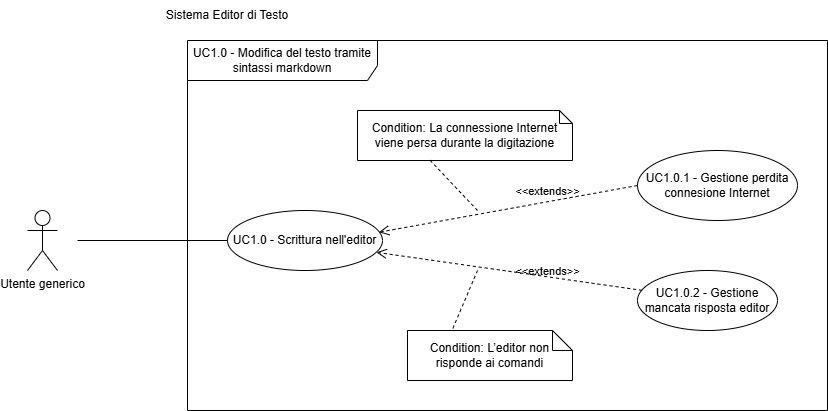
\includegraphics[width=0.8\textwidth]{../UCimg/UC1.0.jpg}
    \caption{Diagramma dei casi d'uso UC-1.0, 1.0.1, 1.0.2}
    \label{fig:uc1.0}
\end{figure}

\subsubsection{UC-1.1 - Visualizzazione anteprima in tempo reale}
\begin{itemize}
    \item \textbf{Attore principale}: Utente generico
    \item \textbf{Descrizione}: Visualizzazione in tempo reale del testo formattato
    \item \textbf{Precondizioni}: L'editor contiene testo con sintassi \gls{Markdown}
    \item \textbf{Postcondizioni}: Viene visualizzata l'anteprima formattata del testo in un'area apposita
    \item \textbf{Scenario principale}:
        \begin{itemize}
            \item L'utente sta digitando testo nell'editor
            \item Il sistema elabora la sintassi \gls{Markdown}
            \item Il sistema aggiorna il pannello di preview mostrando l’anteprima formattata del documento
            \item L'utente può confrontare editing e risultato finale
        \end{itemize}
    \item \textbf{Estensioni}:
        \begin{itemize}
            \item L'anteprima non si aggiorna correttamente
        \end{itemize}
\end{itemize}

\subsubsection{UC-1.1.1 - Gestione errore nell'anteprima}
\begin{itemize}
    \item \textbf{Attore principale}: Utente generico
    \item \textbf{Descrizione}: L'utente ha scritto del testo ma la sezione di anteprima non si aggiorna correttamente
    \item \textbf{Precondizioni}: L'utente ha scritto del testo
    \item \textbf{Postcondizioni}: Il sistema informa l'utente e mostra un messaggio di errore
    \item \textbf{Scenario principale}:
        \begin{itemize}
            \item L'utente sta digitando testo nell'editor
            \item La sezione di anteprima non si aggiorna correttamente
            \item Il sistema informa l'utente con un messaggio di errore
        \end{itemize}
\end{itemize}

\begin{figure}[H]
    \centering
    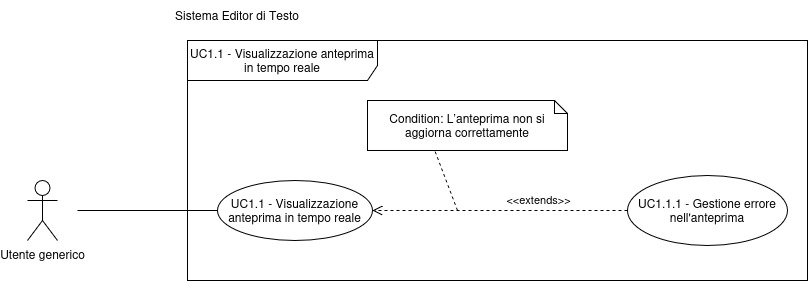
\includegraphics[width=0.8\textwidth]{../UCimg/UC1.1.jpg}
    \caption{Diagramma dei casi d'uso UC-1.1, 1.1.1}
    \label{fig:uc1.1}
\end{figure}

\subsubsection{UC-1.2 - Selezione del testo}
\begin{itemize}
    \item \textbf{Attore principale}: Utente generico
    \item \textbf{Descrizione}: Selezione di porzioni di testo nell’editor
    \item \textbf{Precondizioni}: È presente testo nell'editor
    \item \textbf{Postcondizioni}: Una porzione di testo viene selezionata dall’utente
    \item \textbf{Scenario principale}:
        \begin{itemize}
            \item L'utente evidenzia una porzione di testo con mouse o tastiera
        \end{itemize}
\end{itemize}

\begin{figure}[H]
    \centering
    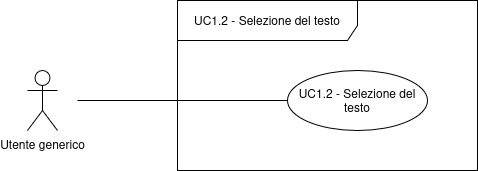
\includegraphics[width=0.8\textwidth]{../UCimg/UC1.2.jpg}
    \caption{Diagramma dei casi d'uso UC-1.2}
    \label{fig:uc1.2}
\end{figure}

\subsubsection{UC-1.3 - Copiare il testo}
\begin{itemize}
    \item \textbf{Attore principale}: Utente generico
    \item \textbf{Descrizione}: L'utente copia una parte di testo dall'area di modifica testo
    \item \textbf{Precondizioni}: Testo presente e selezionato
    \item \textbf{Postcondizioni}: L'utente ha copiato il testo da lui selezionato
    \item \textbf{Scenario principale}:
        \begin{itemize}
            \item L'utente utilizza il comando "Copia" tramite:
                \begin{enumerate}
                    \item Tasto di scelta rapida (Ctrl+C)
                    \item Menu contestuale (tasto destro)
                    \item \gls{Toolbar} dell'editor
                \end{enumerate}
            \item Il testo selezionato viene copiato negli appunti di sistema
            \item Il sistema manda un messaggio di successo
        \end{itemize}
\end{itemize}

\subsubsection{UC-1.4 - Incollare il testo}
\begin{itemize}
    \item \textbf{Attore principale}: Utente generico
    \item \textbf{Descrizione}: L'utente incolla una parte di testo nell'area di modifica testo
    \item \textbf{Precondizioni}: Testo presente negli appunti di sistema
    \item \textbf{Postcondizioni}: L'utente ha incollato il testo precedentemente copiato
    \item \textbf{Scenario principale}:
        \begin{itemize}
            \item L'utente posiziona il cursore nel punto desiderato
            \item L'utente utilizza il comando "Incolla" tramite:
                \begin{enumerate}
                    \item Tasto di scelta rapida (Ctrl+V)
                    \item Menu contestuale (tasto destro)
                    \item \gls{Toolbar} dell'editor (opzionale)
                \end{enumerate}
            \item Il testo dagli appunti viene inserito nella posizione del cursore
        \end{itemize}
\end{itemize}

\subsubsection{UC-1.5 - Tagliare il testo}
\begin{itemize}
    \item \textbf{Attore principale}: Utente generico
    \item \textbf{Descrizione}: L'utente taglia una parte di testo dall'area di modifica, rimuovendola dal documento e copiandola negli appunti
    \item \textbf{Precondizioni}: Testo presente e selezionato
    \item \textbf{Postcondizioni}: Il testo selezionato viene rimosso dall'editor e salvato negli appunti di sistema
    \item \textbf{Scenario principale}:
        \begin{itemize}
            \item L'utente utilizza il comando "Taglia" tramite:
                \begin{enumerate}
                    \item Tasto di scelta rapida (Ctrl+X)
                    \item Menu contestuale (tasto destro)
                    \item \gls{Toolbar} dell'editor (opzionale)
                \end{enumerate}
            \item Il sistema rimuove il testo selezionato dall'editor
            \item Il testo rimosso viene salvato negli appunti di sistema
            \item Il sistema manda un messaggio di successo
        \end{itemize}
\end{itemize}

\begin{figure}[H]
    \centering
    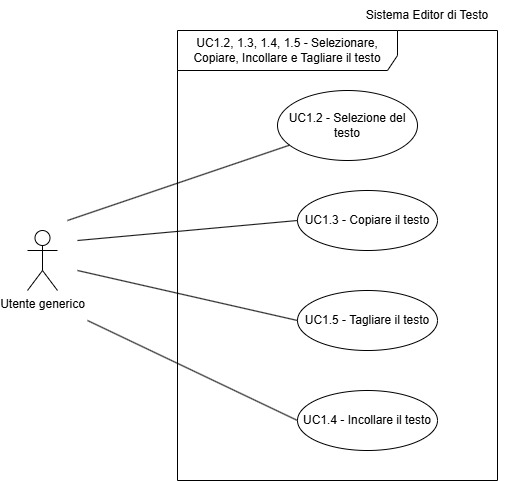
\includegraphics[width=0.8\textwidth]{../UCimg/UC1.3_1.5.jpg}
    \caption{Diagramma dei casi d'uso UC-1.2, 1.3, 1.4, 1.5}
    \label{fig:uc1.3}
\end{figure}

\subsubsection{UC-1.6 - Annullamento modifica (Undo)}
\begin{itemize}
    \item \textbf{Attore principale}: Utente generico
    \item \textbf{Descrizione}: Annullamento dell'ultima operazione di modifica effettuata
    \item \textbf{Precondizioni}: È stata effettuata almeno una modifica al testo e l'utente desidera annullare l'ultima operazione eseguita
    \item \textbf{Postcondizioni}: Il testo ritorna allo stato precedente l'ultima modifica
    \item \textbf{Scenario principale}:
        \begin{itemize}
            \item L'utente effettua una modifica al testo che non soddisfa le sue aspettative
            \item L'utente seleziona l'opzione "Annulla" tramite:
                \begin{enumerate}
                    \item Tasto di scelta rapida (Ctrl+Z)
                    \item Pulsante nella \gls{toolbar} dell'editor (freccia verso sinistra)
                \end{enumerate}
            \item Il sistema ripristina il testo allo stato precedente la modifica
            \item L'operazione annullata viene spostata nella coda redo
        \end{itemize}
    \item \textbf{Estensioni}:
        \begin{itemize}
            \item Non ci sono operazioni da annullare
        \end{itemize}
\end{itemize}

\subsubsection{UC-1.6.1 - Gestione assenza di modifiche annullabili}
\begin{itemize}
    \item \textbf{Attore principale}: Utente generico
    \item \textbf{Descrizione}: L'utente tenta di annullare un'operazione quando non ci sono modifiche anullabili
    \item \textbf{Precondizioni}: L'utente non ha effettuato modifiche anullabili
    \item \textbf{Postcondizioni}: Il documento rimane invariato
    \item \textbf{Scenario principale}:
        \begin{itemize}
            \item L'utente tenta di selezionare l'opzione "Annulla"
            \item Il sistema informa l'utente con un messaggio
            \item Il comando undo non modifica il documento
        \end{itemize}
\end{itemize}

\subsubsection{UC-1.7 - Ripristino modifica (Redo)}
\begin{itemize}
    \item \textbf{Attore principale}: Utente generico
    \item \textbf{Descrizione}: Ripristino di un'operazione precedentemente annullata
    \item \textbf{Precondizioni}: È stata effettuata almeno un'operazione di undo; l'utente desidera ripristinare un'operazione precedentemente annullata
    \item \textbf{Postcondizioni}: Il testo ritorna allo stato successivo all'operazione ripristinata
    \item \textbf{Scenario principale}:
        \begin{itemize}
            \item L'utente ha annullato una o più operazioni con undo
            \item L'utente decide di ripristinare un'operazione annullata
            \item L'utente seleziona l'opzione "Ripristina" tramite:
                \begin{enumerate}
                    \item Tasto di scelta rapida (Ctrl+Y o Ctrl+Shift+Z)
                    \item Pulsante nella \gls{toolbar} dell'editor
                \end{enumerate}
            \item Il sistema riapplica l'ultima operazione annullata
            \item L'operazione viene rimossa dalla coda redo
        \end{itemize}
    \item \textbf{Estensioni}:
        \begin{itemize}
            \item Non ci sono operazioni da ripristinare
        \end{itemize}
\end{itemize}

\subsubsection{UC-1.7.1 - Errore per modifiche non ripristinabili}
\begin{itemize}
    \item \textbf{Attore principale}: Utente generico
    \item \textbf{Descrizione}: L'utente tenta di ripristinare un'operazione quando non ci sono modifiche ripristinabili
    \item \textbf{Precondizioni}: L'utente non ha effettuato modifiche ripristinabili
    \item \textbf{Postcondizioni}:  Il documento rimane invariato
    \item \textbf{Scenario}:
        \begin{itemize}
            \item L'utente tenta di selezionare l'opzione "Ripristina"
            \item Il sistema informa l'utente con un messaggio
            \item Il comando redo non modifica il documento
        \end{itemize}
\end{itemize}

\begin{figure}[H]
    \centering
    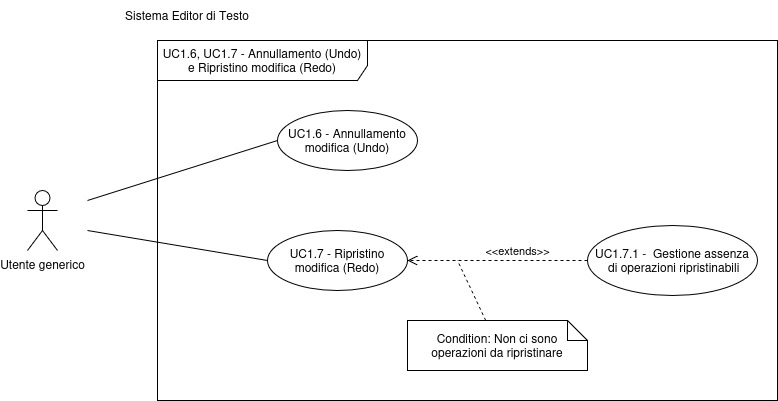
\includegraphics[width=0.8\textwidth]{../UCimg/UC1.6_1.7.jpg}
    \caption{Diagramma dei casi d'uso UC-1.6, 1.7 e estensioni}
    \label{fig:uc1.6}
\end{figure}

\subsubsection{UC-1.8.0 - Modifica del testo selezionato tramite barra degli strumenti}
\begin{itemize}
    \item \textbf{Attore principale}: Utente generico
    \item \textbf{Descrizione}: Formattazione del testo selezionato tramite la barra degli strumenti dell'editor
    \item \textbf{Precondizioni}: È presente testo nell'editor
    \item \textbf{Postcondizioni}: Il testo selezionato viene formattato secondo la sintassi \gls{Markdown}
    \item \textbf{Scenario principale}:
        \begin{itemize}
            \item L'utente seleziona il testo da formattare
            \item L'utente clicca sul pulsante desiderato nella barra degli strumenti
            \item Il sistema applica automaticamente la sintassi \gls{Markdown} corrispondente al testo selezionato
            \item Il testo formattato viene visualizzato nell'area di anteprima
        \end{itemize}
\end{itemize}

\subsubsection{UC-1.8.0.1 - Estensione formattazione a testo parzialmente formattato}
\begin{itemize}
    \item \textbf{Attore principale}: Utente generico
    \item \textbf{Descrizione}: Quando l'utente applica una formattazione a una selezione di testo che la contiene solo parzialmente, il sistema estende la formattazione all'intera selezione anziché rimuoverla
    \item \textbf{Precondizioni}: L'utente ha selezionato una porzione di testo parzialmente formattata
    \item \textbf{Postcondizioni}: L'intera selezione risulta formattata uniformemente con la formattazione applicata
    \item \textbf{Scenario principale}:
        \begin{itemize}
            \item L'utente seleziona una porzione di testo parzialmente formattata
            \item L'utente clicca sul pulsante della formattazione desiderata nella \gls{toolbar}
            \item Il sistema rileva che la selezione contiene solo parzialmente quella formattazione
            \item Il sistema applica la formattazione all'intera selezione
        \end{itemize}
\end{itemize}

\subsubsection{UC-1.8.1 - Rimozione formattazione tramite \gls{toolbar}}
\begin{itemize}
    \item \textbf{Attore principale}: Utente generico
    \item \textbf{Descrizione}: L'utente riapplica la stessa formattazione a una porzione di testo
    \item \textbf{Precondizioni}: Il testo selezionato è formattato
    \item \textbf{Postcondizioni}: Il testo perde quella formattazione
    \item \textbf{Scenario principale}:
        \begin{itemize}
            \item L'utente seleziona il testo formattato
            \item L'utente clicca sul pulsante della stessa formattazione nella \gls{toolbar}
            \item Il sistema rimuove la formattazione dal testo selezionato
        \end{itemize}
\end{itemize}

\begin{figure}[H]
    \centering
    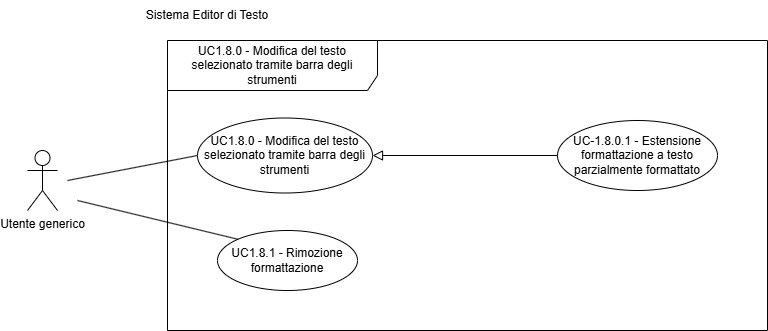
\includegraphics[width=0.8\textwidth]{../UCimg/UC1.8.0.1.jpg}
    \caption{Diagramma dei casi d'uso UC-1.8.0, 1.8.0.1, 1.8.1}
    \label{fig:uc1.8.0}
\end{figure}

\subsubsection{UC-1.8.2 - Applicazione grassetto al testo selezionato}
\begin{itemize}
    \item \textbf{Attore principale}: Utente generico
    \item \textbf{Descrizione}: Formattazione del testo selezionato in grassetto tramite barra degli strumenti
    \item \textbf{Precondizioni}: È presente testo selezionato nell'editor
    \item \textbf{Postcondizioni}: Il testo selezionato viene formattato in grassetto
    \item \textbf{Scenario principale}:
        \begin{itemize}
            \item L'utente seleziona il testo da rendere in grassetto
            \item L'utente clicca sul pulsante "Grassetto" nella \gls{toolbar}
            \item Il sistema applica la sintassi \gls{Markdown} per il grassetto
            \item Il testo viene visualizzato in grassetto nell'anteprima
        \end{itemize}
\end{itemize}

\subsubsection{UC-1.8.3 - Applicazione corsivo al testo selezionato}
\begin{itemize}
    \item \textbf{Attore principale}: Utente generico
    \item \textbf{Descrizione}: Formattazione del testo selezionato in corsivo tramite barra degli strumenti
    \item \textbf{Precondizioni}: È presente testo selezionato nell'editor
    \item \textbf{Postcondizioni}: Il testo selezionato viene formattato in corsivo
    \item \textbf{Scenario principale}:
        \begin{itemize}
            \item L'utente seleziona il testo da rendere in corsivo
            \item L'utente clicca sul pulsante "Corsivo" nella \gls{toolbar}
            \item Il sistema applica la sintassi \gls{Markdown} per il corsivo
            \item Il testo viene visualizzato in corsivo nell'anteprima
        \end{itemize}
\end{itemize}

\subsubsection{UC-1.8.4 - Applicazione sottolineatura al testo selezionato}
\begin{itemize}
    \item \textbf{Attore principale}: Utente generico
    \item \textbf{Descrizione}: Formattazione del testo selezionato come sottolineato tramite barra degli strumenti
    \item \textbf{Precondizioni}: È presente testo selezionato nell'editor
    \item \textbf{Postcondizioni}: Il testo selezionato viene formattato come sottolineato
    \item \textbf{Scenario principale}:
        \begin{itemize}
            \item L'utente seleziona il testo da rendere sottolineato
            \item L'utente clicca sul pulsante "Sottolineato" nella \gls{toolbar}
            \item Il sistema applica la sintassi \gls{Markdown} per sottolineare il testo
            \item Il testo viene visualizzato sottolineato nell'anteprima
        \end{itemize}
\end{itemize}

\subsubsection{UC-1.8.5 - Applicazione intestazioni al testo selezionato}
\begin{itemize}
    \item \textbf{Attore principale}: Utente generico
    \item \textbf{Descrizione}: Applicazione di intestazioni al testo selezionato
    \item \textbf{Precondizioni}: È presente testo selezionato nell’editor
    \item \textbf{Postcondizioni}: Vengono applicate intestazioni al documento
    \item \textbf{Scenario principale}:
        \begin{itemize}
            \item L'utente posiziona il cursore dove inserire l'intestazione
            \item L'utente scrive un'intestazione tramite:
                \begin{enumerate}
                    \item \gls{Toolbar} (H1, H2, H3, ecc.)
                    \item Sintassi \gls{Markdown} (\#, \#\#, \#\#\#)
                \end{enumerate}
            \item Il sistema formatta il testo come intestazione
            \item Le intestazioni vengono visualizzate nell'anteprima
        \end{itemize}
\end{itemize}

\subsubsection{UC-1.8.6 - Inserimento elementi di struttura}
\begin{itemize}
    \item \textbf{Attore principale}: Utente generico
    \item \textbf{Descrizione}: Applicazione di elementi di struttura al documento nel testo selezionato
    \item \textbf{Precondizioni}: È presente testo selezionato nell’editor
    \item \textbf{Postcondizioni}: Vengono applicati gli elementi di struttura selezionati al documento
    \item \textbf{Scenario principale}:
        \begin{itemize}
            \item L’utente posiziona il cursore dove inserire l’elemento di struttura
            \item L’utente sceglie il tipo di struttura da applicare:
                \begin{enumerate}
                    \item Tabella
                    \item Separatore orizzontale
                \end{enumerate}
            \item Gli elementi formattati vengono visualizzati nell'anteprima
        \end{itemize}
\end{itemize}

\subsubsection{UC-1.8.7 - Inserimento di liste ed elenchi}
\begin{itemize}
    \item \textbf{Attore principale}: Utente generico
    \item \textbf{Descrizione}: Creazione di liste ordinate e non ordinate nel documento da testo selezionato o non selezionato
    \item \textbf{Precondizioni}: L'editor è aperto e funzionante
    \item \textbf{Postcondizioni}: Viene creata una lista ordinata o non ordinata
    \item \textbf{Scenario principale}:
        \begin{itemize}
            \item L'utente posiziona il cursore nel punto dove vuole inserire la lista
            \item L'utente seleziona il tipo di lista (ordinata/non ordinata)
            \item L'utente inserisce gli elementi della lista
            \item Il sistema formatta automaticamente la lista
            \item La lista formattata viene visualizzata nell'anteprima
        \end{itemize}
\end{itemize}

\subsubsection{UC-1.8.7.1 - Gestione di sotto-liste}
\begin{itemize}
    \item \textbf{Attore principale}: Utente generico
    \item \textbf{Descrizione}: L'utente vuole inserire una sotto-lista all'interno di una lista esistente
    \item \textbf{Precondizioni}: È presente una lista nell'editor
    \item \textbf{Postcondizioni}: Viene inserita una sotto-lista all'interno della lista esistente
    \item \textbf{Scenario principale}:
        \begin{itemize}
            \item L'utente inizializza una lista indentata dentro ad un'altra
            \item Il sistema crea una sottolista
            \item Il sistema gestisce l'indentazione automatica della nuova sotto-lista
            \item La sotto-lista formattata viene visualizzata correttamente nell'anteprima
        \end{itemize}
\end{itemize}

\subsubsection{UC-1.8.8 - Inserimento di link e riferimenti}
\begin{itemize}
    \item \textbf{Attore principale}: Utente generico
    \item \textbf{Descrizione}: Inserimento di link ipertestuali al testo selezionato nel documento
    \item \textbf{Precondizioni}: È presente testo da collegare o l'utente vuole inserire un link
    \item \textbf{Postcondizioni}: Viene inserito un link ipertestuale nel documento
    \item \textbf{Scenario principale}:
        \begin{itemize}
            \item L'utente seleziona il testo da trasformare in link
            \item L'utente clicca sul comando "Inserisci link"
            \item L'utente inserisce l'URL di destinazione
            \item Il sistema applica la sintassi \gls{Markdown} per il link
            \item Il link viene visualizzato con la formattazione corretta nell'anteprima
        \end{itemize}
\end{itemize}

\begin{figure}[H]
    \centering
    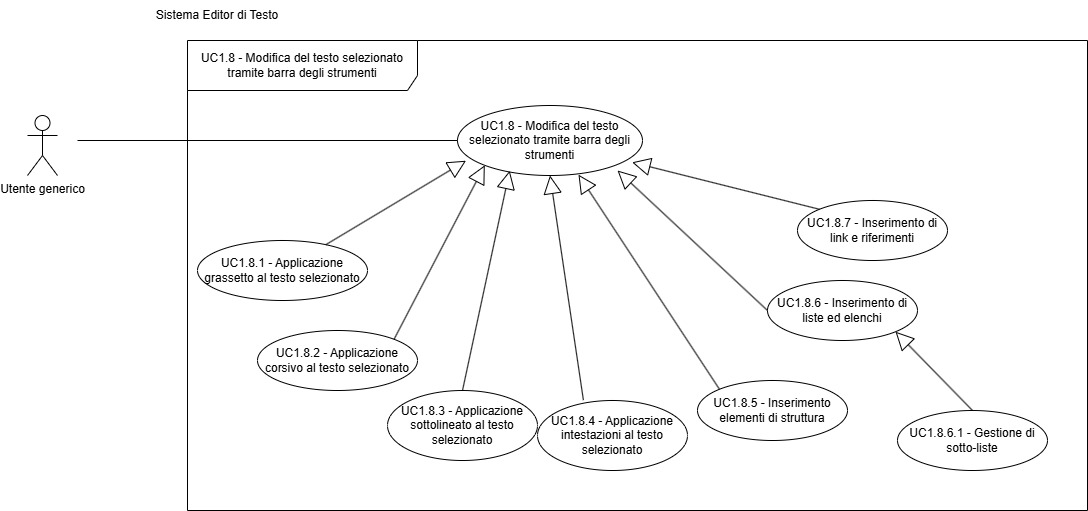
\includegraphics[width=0.8\textwidth]{../UCimg/UC1.8.jpg}
    \caption{Diagramma dei casi d'uso UC-1.8.*}
    \label{fig:uc1.8}
\end{figure}

\subsubsection{UC-1.9 - Impostare formattazioni senza testo presente nell'editor}
\begin{itemize}
    \item \textbf{Attore principale}: Utente generico
    \item \textbf{Descrizione}: Applicazione di formattazioni tramite barra degli strumenti senza che l'utente abbia già digitato del testo nell'editor
    \item \textbf{Precondizioni}: L’editor è aperto e l'utente ha accesso agli strumenti di formattazione
    \item \textbf{Postcondizioni}: Il testo futuro viene formattato in base alla formattazione già selezionata dall'utente prima della scrittura di testo 
    \item \textbf{Scenario principale}:
        \begin{itemize}
            \item L’utente seleziona la formattazione per il testo futuro
            \item Il sistema applica la sintassi \gls{Markdown} corrispondente, anche in caso di multiple formattazioni
            \item Il testo scritto dall'utente prende la formattazione applicata
        \end{itemize}
\end{itemize}

\subsubsection{UC-1.9.1 - Impostare grassetto al testo futuro}
\begin{itemize}
    \item \textbf{Attore principale}: Utente generico
    \item \textbf{Descrizione}: Formattazione del testo futuro scritto dall’utente in grassetto
    \item \textbf{Precondizioni}: L’utente ha accesso alla formattazione in grassetto
    \item \textbf{Postcondizioni}: Il testo scritto è in grassetto
    \item \textbf{Scenario principale}:
        \begin{itemize}
            \item L’utente clicca sul pulsante "Grassetto" nella \gls{toolbar}
            \item Il sistema applica la sintassi \gls{Markdown} per il grassetto
            \item Il testo scritto successivamente dall'utente prende automaticamente la formattazione in grassetto
            \item Il testo in grassetto viene visualizzato correttamente nell'anteprima
        \end{itemize}
\end{itemize}

\subsubsection{UC-1.9.2 - Impostare corsivo al testo futuro}
\begin{itemize}
    \item \textbf{Attore principale}: Utente generico
    \item \textbf{Descrizione}: Formattazione del testo futuro scritto dall’utente in corsivo
    \item \textbf{Precondizioni}: L’utente ha accesso alla formattazione in corsivo
    \item \textbf{Postcondizioni}: Il testo scritto è in corsivo
    \item \textbf{Scenario principale}:
        \begin{itemize}
            \item L’utente clicca sul pulsante "Corsivo" nella \gls{toolbar}
            \item Il sistema applica la sintassi \gls{Markdown} per il corsivo
            \item Il testo scritto successivamente dall'utente prende automaticamente la formattazione in corsivo
            \item Il testo in corsivo viene visualizzato correttamente nell'anteprima
        \end{itemize}
\end{itemize}

\subsubsection{UC-1.9.3 - Impostare sottolineatura al testo futuro}
\begin{itemize}
    \item \textbf{Attore principale}: Utente generico
    \item \textbf{Descrizione}: Formattazione del testo futuro scritto dall’utente in modalità sottolineata

    \item \textbf{Precondizioni}: L’utente ha accesso alla formattazione sottolineata
    \item \textbf{Postcondizioni}: Il testo scritto è sottolineato
    \item \textbf{Scenario principale}:
        \begin{itemize}
            \item L’utente clicca sul pulsante "Sottolineato" nella \gls{toolbar}
            \item Il sistema applica la sintassi \gls{Markdown} per la sottolineatura
            \item Il testo scritto successivamente dall'utente prende automaticamente la sottolineatura
            \item Il testo sottolineato viene visualizzato correttamente nell'anteprima
        \end{itemize}
\end{itemize}

\subsubsection{UC-1.9.4 - Impostare intestazioni}
\begin{itemize}
    \item \textbf{Attore principale}: Utente generico
    \item \textbf{Descrizione}: Formattazione del testo futuro scritto dall’utente rispettando le intestazioni
    \item \textbf{Precondizioni}: L’utente ha accesso alla formattazione per le intestazioni
    \item \textbf{Postcondizioni}: Il testo scritto presenta le intestazioni
    \item \textbf{Scenario principale}:
        \begin{itemize}
            \item L’utente clicca sul pulsante "Intestazioni" nella \gls{toolbar}
            \item L’utente applica un’intestazione tramite:
                \begin{enumerate}
                    \item \gls{Toolbar} (H1, H2, H3, ecc.)
                    \item Sintassi \gls{Markdown} (\#, \#\#, \#\#\#)
                \end{enumerate}
            \item Il testo scritto successivamente dall'utente prende automaticamente la formattazione dell'intestazione
            \item L'intestazione viene visualizzata correttamente nell'anteprima
        \end{itemize}
\end{itemize}

\subsubsection{UC-1.9.5 - Impostare struttura al documento}
\begin{itemize}
    \item \textbf{Attore principale}: Utente generico
    \item \textbf{Descrizione}: Formattazione del testo futuro scritto dall’utente secondo una struttura da lui selezionata
    \item \textbf{Precondizioni}: L’utente ha accesso alla formattazione per la gestione della struttura
    \item \textbf{Postcondizioni}: Il testo scritto rispetta la struttura selezionata dall’utente
    \item \textbf{Scenario principale}:
        \begin{itemize}
            \item L’utente clicca sul pulsante "Struttura" nella \gls{toolbar}
            \item L’utente sceglie il tipo di struttura da applicare:
                \begin{enumerate}
                    \item Tabella
                    \item Separatore orizzontale
                \end{enumerate}
            \item L'elemento viene visualizzato correttamente nell'anteprima
        \end{itemize}
\end{itemize}

\subsubsection{UC-1.9.6 - Impostare liste ed elenchi}
\begin{itemize}
    \item \textbf{Attore principale}: Utente generico
    \item \textbf{Descrizione}: Formattazione del testo futuro scritto dall’utente secondo una lista o un elenco
    \item \textbf{Precondizioni}: L’utente ha accesso alla formattazione per la gestione delle liste ed elenchi
    \item \textbf{Postcondizioni}: Il testo scritto è in formato lista/elenco
    \item \textbf{Scenario principale}:
        \begin{itemize}
            \item L’utente clicca sul pulsante "Liste ed elenchi" nella \gls{toolbar}
            \item L’utente sceglie il tipo di elenco da applicare:
                \begin{itemize}
                    \item ordinato/non ordinato
                \end{itemize}
            \item La formattazione viene applicata e l'utente può inserire testo nella lista già pronta
            \item La lista viene visualizzata correttamente nell'anteprima
        \end{itemize}
\end{itemize}

\subsubsection{UC-1.9.7 - Impostare link e riferimenti}
\begin{itemize}
    \item \textbf{Attore principale}: Utente generico
    \item \textbf{Descrizione}: Formattazione per l’inserimento dei link o riferimenti
    \item \textbf{Precondizioni}:L’utente ha accesso alla formattazione per la gestione dei link e riferimenti
    \item \textbf{Postcondizioni}:Il testo scritto è un link/riferimento
    \item \textbf{Scenario principale}:
        \begin{itemize}
            \item L’utente clicca sul comando ”Inserisci link o riferimento”
            \item L’utente inserisce l’URL di destinazione
            \item Il sistema applica la sintassi \gls{Markdown} per il link o riferimenti
            \item Il link viene visualizzato correttamente nell'anteprima
        \end{itemize}
\end{itemize}

\begin{figure}[H]
    \centering
    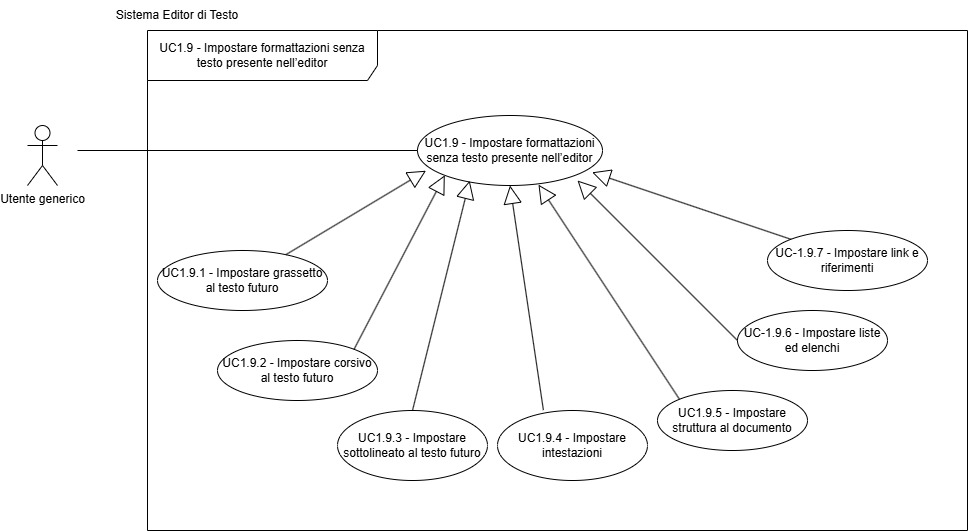
\includegraphics[width=0.8\textwidth]{../UCimg/UC1.9.jpg}
    \caption{Diagramma dei casi d'uso UC-1.9.*}
    \label{fig:uc1.9}
\end{figure}

\subsubsection{UC-1.10 - Gestione modalità di visualizzazione}
\begin{itemize}
    \item \textbf{Attore principale}: Utente generico
    \item \textbf{Descrizione}: Selezione della modalità di visualizzazione dell’area di lavoro per alternare tra scrittura, anteprima o visione combinata
    \item \textbf{Precondizioni}: L’editor è aperto e funzionante
    \item \textbf{Postcondizioni}: L’interfaccia viene adattata alla modalità di visualizzazione selezionata
    \item \textbf{Scenario principale}:
        \begin{itemize}
            \item L’utente accede ai comandi di visualizzazione
            \item L’utente seleziona la modalità di visualizzazione desiderata tra quelle disponibili
            \item Il sistema riconfigura i pannelli dell'interfaccia in base alla scelta effettuata
        \end{itemize}
\end{itemize}

\subsubsection{UC-1.10.1 - Modalità di visualizzazione solo editor}
\begin{itemize}
    \item \textbf{Attore principale}: Utente generico
    \item \textbf{Descrizione}: Cambia la modalità di visualizzazione dell’editor, che mostra solo l'area di scrittura dell'editor
    \item \textbf{Precondizioni}: La modalità di visualizzazione comprende solo il documento formattato oppure è in modalità split view
    \item \textbf{Postcondizioni}: Visualizzazione esclusiva dell'area di testo dell'editor
    \item \textbf{Scenario principale}:
        \begin{itemize}
            \item L'utente seleziona la modalità di visualizzazione "Solo editor" (sintassi \gls{Markdown} visibile)
            \item Il sistema adatta l'interfaccia alla modalità scelta
        \end{itemize}
\end{itemize}


\subsubsection{UC-1.10.2 - Modalità di visualizzazione solo documento formattato}
\begin{itemize}
    \item \textbf{Attore principale}: Utente generico
    \item \textbf{Descrizione}: Cambia la modalità di visualizzazione dell'editor, che mostra solo l'anteprima formattata del documento
    \item \textbf{Precondizioni}: La modalità di visualizzazione comprende solo l’editor oppure è in modalità split view
    \item \textbf{Postcondizioni}: Visualizzazione esclusiva del documento formattato
    \item \textbf{Scenario principale}:
        \begin{itemize}
            \item L'utente seleziona la modalità di visualizzazione "Solo documento"/"Solo anteprima"
            \item Il sistema adatta l'interfaccia alla modalità scelta
        \end{itemize}
\end{itemize}

\subsubsection{UC-1.10.3 - Modalità di visualizzazione split view}
\begin{itemize}
    \item \textbf{Attore principale}: Utente generico
    \item \textbf{Descrizione}: Cambia la modalità di visualizzazione in split view, che mostra sia l'area di testo sia l'anteprima del documento formattato
    \item \textbf{Precondizioni}: La modalità di visualizzazione comprende solo l’editor oppure solo il documento
    \item \textbf{Postcondizioni}: Visualizzazione split view dell’area di testo e del documento formattato
    \item \textbf{Scenario principale}:
        \begin{itemize}
            \item L'utente seleziona la modalità di visualizzazione "Split View"
            \item Il sistema adatta l'interfaccia alla modalità scelta
        \end{itemize}
\end{itemize}

\begin{figure}[H]
    \centering
    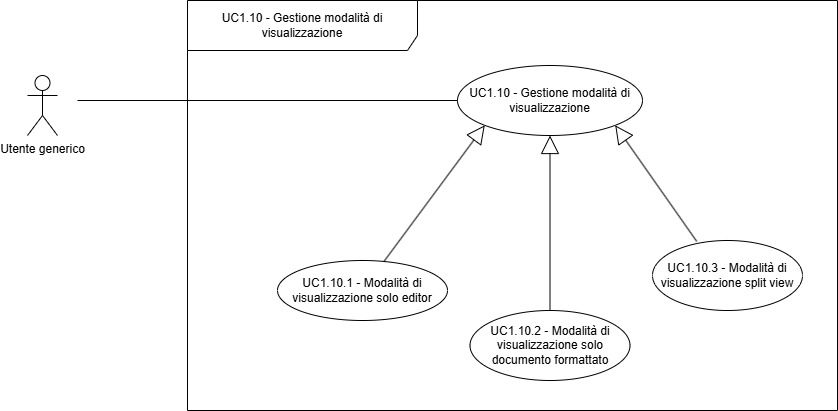
\includegraphics[width=0.8\textwidth]{../UCimg/UC1.10.jpg}
    \caption{Diagramma dei casi d'uso UC-1.10, 1.10.*}
    \label{fig:uc1.10}
\end{figure}

\subsubsection{UC-1.11 - Ricerca di caratteri nel testo}
\begin{itemize}
    \item \textbf{Attore principale}: Utente generico
    \item \textbf{Descrizione}: Ricerca di occorrenze di una stringa di testo all'interno del documento tramite corrispondenza esatta e non 
    case-sensitive.
    \item \textbf{Precondizioni}: È presente testo nell'editor
    \item \textbf{Postcondizioni}: Le occorrenze della stringa cercata 
    vengono evidenziate nel testo
    \item \textbf{Scenario principale}:
        \begin{itemize}
            \item L'utente attiva la funzione "Ricerca"
            \item L'utente inserisce la stringa di testo da cercare
            \item Il sistema cerca tutte le occorrenze esatte della stringa nel documento in modo non case-sensitive
            \item Il sistema evidenzia simultaneamente tutte le occorrenze 
            trovate nel testo
        \end{itemize}
    \item \textbf{Estensioni}:
        \begin{itemize}
            \item Nessuna occorrenza trovata
        \end{itemize}
\end{itemize}

\subsubsection{UC-1.11.1 - Gestione assenza di occorrenze}
\begin{itemize}
    \item \textbf{Attore principale}: Utente generico
    \item \textbf{Descrizione}: La ricerca non trova occorrenze di testo nell'editor
    \item \textbf{Precondizioni}: L'utente effettua una ricerca
    \item \textbf{Postcondizioni}: L'utente viene informato che nessuna occorrenza è stata trovata
    \item \textbf{Scenario}:
        \begin{itemize}
            \item L'utente attiva la funzione "Ricerca"
            \item L'utente inserisce il testo da cercare
            \item Il sistema non trova occorrenze
            \item Il sistema informa l'utente che nessuna occorrenza è stata trovata con un messaggio
        \end{itemize}
\end{itemize}

\begin{figure}[H]
    \centering
    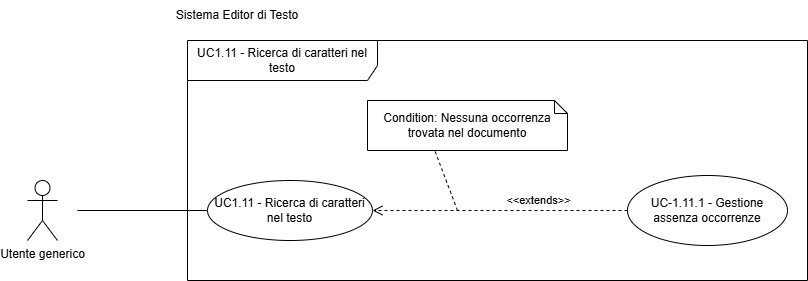
\includegraphics[width=0.8\textwidth]{../UCimg/UC1.11.jpg}
    \caption{Diagramma dei casi d'uso UC-1.11, 1.11.1}
    \label{fig:uc1.11}
\end{figure}

\newpage

\subsection{Macroarea 2 - Funzionalità AI}
\subsubsection{UC-2.0 - Visualizzazione storico generazioni AI}
\begin{itemize}
    \item \textbf{Attore principale}: Utente generico
    \item \textbf{Descrizione}: L'utente visualizza il registro delle generazioni AI effettuate nel documento corrente
    \item \textbf{Precondizioni}: Sono state eseguite una o più operazioni AI nel documento corrente
    \item \textbf{Postcondizioni}: L’utente visualizza il registro delle generazioni AI
    \item \textbf{Scenario principale}:
        \begin{itemize}
            \item L’utente seleziona l’opzione “Visualizza storico generazioni"
            \item Il sistema mostra un registro con tutte le generazioni AI effettuate nel documento
            \item Per ogni voce il sistema mostra il titolo e il testo generato
        \end{itemize}
        \item \textbf{Estensioni}:
        \begin{itemize}
            \item Il registro delle generazioni è vuoto
        \end{itemize}
\end{itemize}

\subsubsection{UC-2.0.1 - Visualizzazione storico generazioni vuoto}
\begin{itemize}
    \item \textbf{Attore principale}: Utente generico
    \item \textbf{Descrizione}: L'utente accede allo storico ma non sono presenti generazioni AI
    \item \textbf{Precondizioni}: L'utente ha selezionato "Visualizza storico generazioni" e non sono state eseguite operazioni AI nella sessione corrente
    \item \textbf{Postcondizioni}: Il sistema informa l'utente che il registro è vuoto
    \item \textbf{Scenario principale}:
        \begin{itemize}
            \item L'utente seleziona "Visualizza storico generazioni"
            \item Il sistema rileva che non sono presenti generazioni AI
            \item Il sistema mostra un messaggio informativo
        \end{itemize}
\end{itemize}

\subsubsection{UC-2.0.2 - Visualizzazione titolo generazione}
\begin{itemize}
    \item \textbf{Attore principale}: Utente generico
    \item \textbf{Descrizione}: Per ogni voce dello storico il sistema mostra un titolo che identifica la generazione, composto dal 
    nome della funzionalità AI utilizzata e dalla data e ora della generazione
    \item \textbf{Precondizioni}: Lo storico delle generazioni AI è aperto e contiene almeno una voce
    \item \textbf{Postcondizioni}: Il titolo di ogni generazione è visibile nel registro
    \item \textbf{Scenario principale}:
        \begin{itemize}
            \item Il sistema recupera il titolo della generazione 
            \item Il titolo viene mostrato per ogni voce del registro
        \end{itemize}
\end{itemize}

\subsubsection{UC-2.0.3 - Visualizzazione testo generato}
\begin{itemize}
    \item \textbf{Attore principale}: Utente generico
    \item \textbf{Descrizione}: Per ogni voce dello storico il sistema mostra il testo prodotto dalla generazione AI
    \item \textbf{Precondizioni}: Lo storico delle generazioni AI è aperto e contiene almeno una voce
    \item \textbf{Postcondizioni}: Il testo generato è visibile per ogni voce del registro
    \item \textbf{Scenario principale}:
        \begin{itemize}
            \item Il sistema recupera il testo generato associato alla voce
            \item Il testo viene mostrato per ogni voce del registro
        \end{itemize}
\end{itemize}

\subsubsection{UC-2.0.4 - Eliminazione di una generazione dallo storico generazioni AI}
\begin{itemize}
    \item \textbf{Attore principale}: Utente generico
    \item \textbf{Descrizione}: L'utente elimina una voce dal registro delle generazioni AI
    \item \textbf{Precondizioni}: Lo storico delle generazioni AI è aperto e contiene almeno una voce
    \item \textbf{Postcondizioni}: La voce selezionata viene rimossa dal registro
    \item \textbf{Scenario principale}:
        \begin{itemize}
            \item L'utente seleziona l'opzione "Elimina" associata a una generazione del registro
            \item Il sistema rimuove la voce dal registro
        \end{itemize}
\end{itemize}

\subsubsection{UC-2.0.5 - Visualizzazione storico generazioni AI per utente registrato}
\begin{itemize}
    \item \textbf{Attore principale}: Utente registrato
    \item \textbf{Descrizione}: Lo storico delle generazioni AI è persistente ed è associato ai documenti salvati nell’account dell’utente
    \item \textbf{Precondizioni}: L’utente ha effettuato il log-in e ha eseguito una o più operazioni AI
    \item \textbf{Postcondizioni}: L’utente visualizza il registro delle generazioni AI associate ai documenti salvati nel suo account
    \item \textbf{Scenario principale}:
        \begin{itemize}
            \item L'utente ha effettuato il log-in e ha eseguito una o più operazioni AI
            \item L’utente seleziona l’opzione “Visualizza storico generazioni"
            \item Il sistema mostra un registro con tutte le generazioni AI associate ai documenti salvati nel suo account
        \end{itemize}
\end{itemize}

\begin{figure}[H]
    \centering
    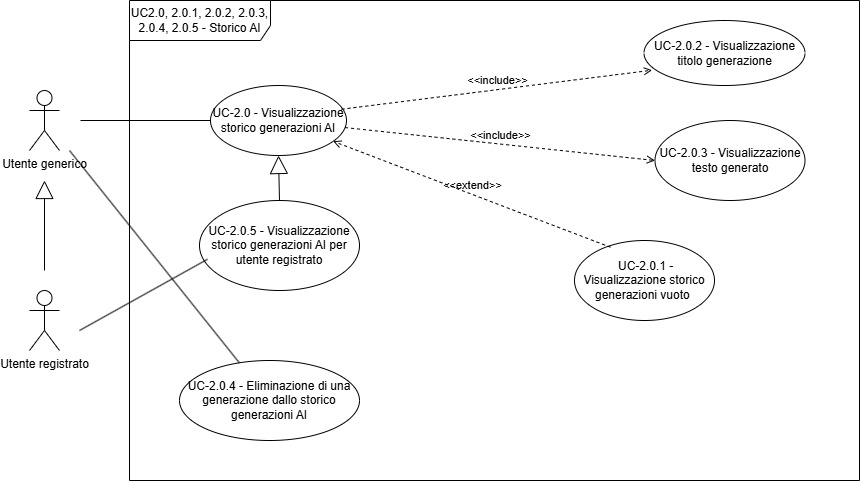
\includegraphics[width=0.8\textwidth]{../UCimg/UC2.0.1.jpg}
    \caption{Diagramma casi d'uso UC-2.0, 2.0.1, 2.0.2, 2.0.3, 2.0.4, 2.0.5}
    \label{fig:da2.0_2.0.5}
\end{figure}

\begin{figure}[H]
    \centering
    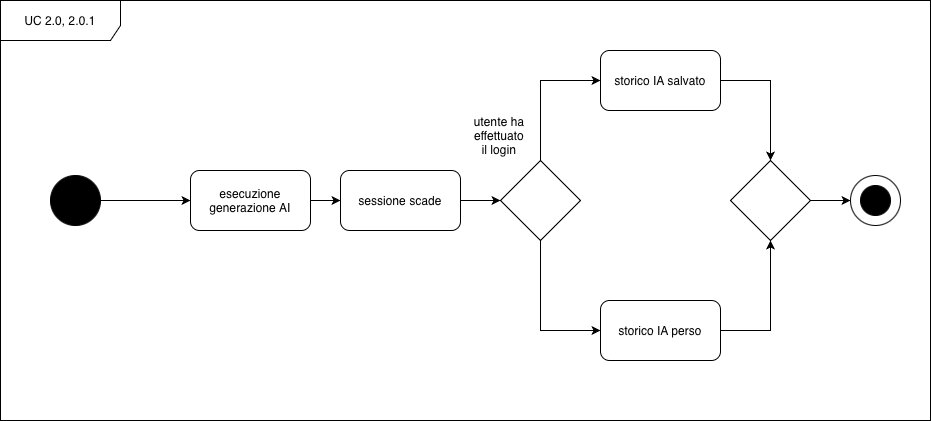
\includegraphics[width=0.8\textwidth]{../UCimg/UC2.0_2.0.1_activity.jpg}
    \caption{Diagramma delle attività UC-2.0, 2.0.1}
    \label{fig:da2.0_2.0.1}
\end{figure}

\subsubsection{UC-2.1 - Interazione con i testi generati dall’AI}
\begin{itemize}
    \item \textbf{Attore principale}: Utente generico
    \item \textbf{Descrizione}: Ogni volta che l’utente effettua un’operazione AI può leggerla e interagire con essa
    \item \textbf{Precondizioni}: E’ stata eseguita un’operazione AI
    \item \textbf{Postcondizioni}: La proposta AI è stata inserita nello storico delle generazioni AI e l'utente ha interagito con essa confermandola, eliminandola o rigenerandola
    \item \textbf{Scenario principale}:
    \begin{itemize}
        \item L'utente avvia un'operazione AI sul testo selezionato o sull'intero documento
        \item Il sistema comunica con il servizio LLM e attende la risposta
        \item Il sistema mostra la proposta generata distinta visivamente dal testo dell'utente
        \item L'utente interagisce con la proposta
        \item La generazione viene inserita nello storico delle generazioni AI
    \end{itemize}
    \item \textbf{Estensioni}:
    \begin{itemize}
        \item Il servizio LLM restituisce un errore senza dare risposta
    \end{itemize}
\end{itemize}

\begin{figure}[H]
    \centering
    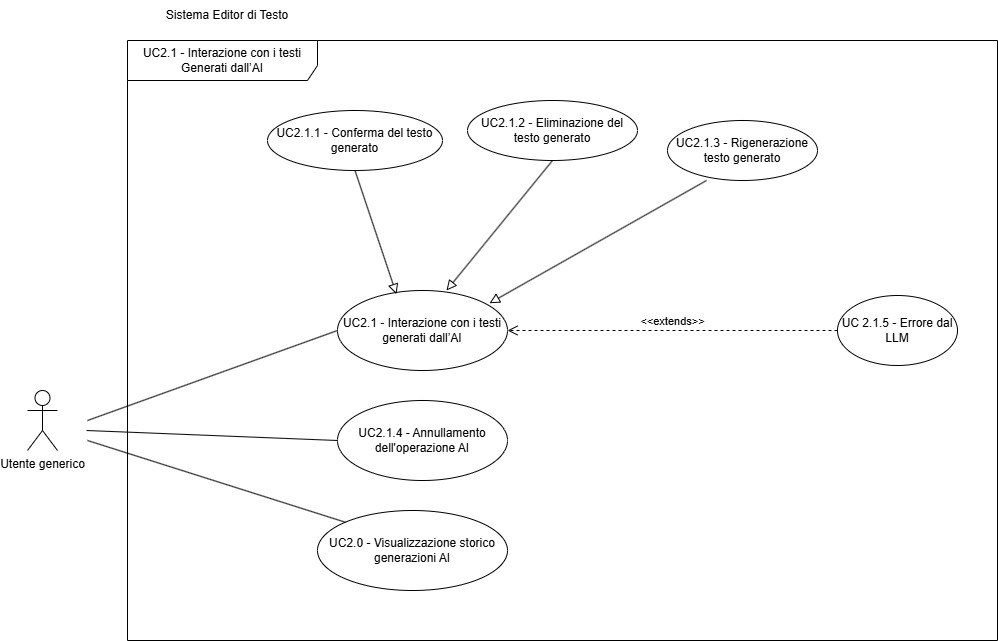
\includegraphics[width=0.8\textwidth]{../UCimg/UC2.1.jpg}
    \caption{Diagramma dei casi d'uso UC-2.1, 2.1.*}
    \label{fig:uc2.1}
\end{figure}

\subsubsection{UC-2.1.1 - Conferma del testo generato dall'AI}
\begin{itemize}
    \item \textbf{Attore principale}: Utente generico
    \item \textbf{Descrizione}: L’utente accetta la proposta di testo generata dall'AI
    \item \textbf{Precondizioni}: Il foglio di lavoro contiene la proposta di testo generata dall’AI
    \item \textbf{Postcondizioni}: L’utente accetta la proposta di testo generato, che viene successivamente integrata nel documento nell'editor
    \item \textbf{Scenario principale}:
    \begin{itemize}
        \item L’utente visualizza una proposta di testo generata dall’AI
        \item L’utente seleziona l’opzione "Conferma"
        \item Il testo generato viene integrato nel documento aperto nell'editor
    \end{itemize}
\end{itemize}

\subsubsection{UC-2.1.2 - Eliminazione del testo generato}
\begin{itemize}
    \item \textbf{Attore principale}: Utente generico
    \item \textbf{Descrizione}: L’utente può eliminare intere sezioni di testo generato dall’AI
    \item \textbf{Precondizioni}: Sono state eseguite una o più operazioni AI e i relativi testi generati sono stati inseriti nell’editor
    \item \textbf{Postcondizioni}: L’utente elimina il testo generato
    \item \textbf{Scenario principale}:
    \begin{itemize}
        \item L’utente individua un blocco di testo generato dall’AI
        \item L’utente visualizza l’opzione "Annulla" accanto alla generazione
        \item L’utente seleziona “Annulla”
        \item Il testo generato viene cancellato dal documento nell'editor
    \end{itemize}
\end{itemize}

\subsubsection{UC-2.1.3 - Rigenerazione testo generato}
\begin{itemize}
    \item \textbf{Attore principale}: Utente generico
    \item \textbf{Descrizione}: L’utente può rigenerare intere sezioni di testo precedentemente generato dall’AI
    \item \textbf{Precondizioni}: Sono state eseguite una o più operazioni AI e i relativi testi generati sono stati inseriti nell’editor
    \item \textbf{Postcondizioni}: Il testo generato precedentemente viene sostituito da una nuova variante prodotta dall'AI
    \item \textbf{Scenario principale}:
    \begin{itemize}
        \item L’utente individua un blocco di testo generato dall’AI
        \item L’utente visualizza l’opzione “Rigenera” accanto alla generazione
        \item L’utente seleziona “Rigenera”
        \item Il sistema invia nuovamente la richiesta all'AI utilizzando gli stessi parametri
        \item Il testo precedentemente generato viene sovrascritto da una nuova generazione
    \end{itemize}
\end{itemize}

\subsubsection{UC-2.1.4 - Errore dal LLM}
\begin{itemize}
    \item \textbf{Attore principale}: Utente generico
    \item \textbf{Descrizione}: Il sistema gestisce un fallimento nella generazione della risposta da parte del LLM (es. timeout, assenza di connessione, errore server)
    \item \textbf{Precondizioni}: L'utente ha avviato un'operazione AI e il sistema ha qualche errore in fase di elaborazione
    \item \textbf{Postcondizioni}: L’utente viene informato dell'errore e il documento rimane nello stato precedente alla richiesta
    \item \textbf{Scenario principale}:
    \begin{itemize}
        \item Il sistema tenta di comunicare con il servizio LLM esterno
        \item Il servizio LLM non risponde o restituisce un codice di errore
        \item Il sistema riceve l'errore interrompendo il processo di attesa
        \item Il sistema manda un messaggio di errore all'utente
        \item Il testo presente nell’editor rimane invariato
    \end{itemize}
\end{itemize}

\subsubsection{UC-2.1.5 - Annullamento dell’operazione AI}
\begin{itemize}
    \item \textbf{Attore principale}: Utente generico
    \item \textbf{Descrizione}: L’utente interrompe volontariamente una richiesta AI in corso prima del suo completamento
    \item \textbf{Precondizioni}: L'utente ha avviato un'operazione AI e il sistema è in fase di elaborazione
    \item \textbf{Postcondizioni}: L’operazione viene annullata e il documento rimane nello stato precedente alla richiesta
    \item \textbf{Scenario principale}:
    \begin{itemize}
        \item Il sistema sta elaborando una richiesta AI
        \item L’editor mostra un indicatore di attesa (opzionale)
        \item L’utente seleziona l’opzione “Annulla” per l’operazione in corso
        \item L’editor interrompe l’operazione e la comunicazione con il servizio LLM
        \item Il testo presente nell’editor rimane invariato
    \end{itemize}
\end{itemize}

\subsubsection{UC-2.2 - Riassunto del testo}
\begin{itemize}
    \item \textbf{Attore principale}: Utente generico
    \item \textbf{Descrizione}: Generazione di un riassunto del testo selezionato o dell’intero documento
    \item \textbf{Precondizioni}: L’editor contiene del testo
    \item \textbf{Postcondizioni}: Un nuovo blocco di testo contenente il riassunto viene inserito nell’editor, in seguito alla conferma dell'utente
    \item \textbf{Scenario principale}:
    \begin{itemize}
        \item L’utente seleziona una porzione di testo (o non seleziona nulla per indicare l'intero documento)
        \item L’utente attiva il comando ”Riassumi”
        \item Il sistema elabora la richiesta e invia il testo al LLM
        \item Il sistema genera il riassunto
        \item L'utente conferma il riassunto
        \item Il sistema lo inserisce nell'editor
    \end{itemize}
\end{itemize}

\begin{figure}[H]
    \centering
    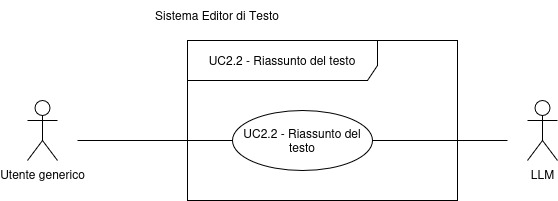
\includegraphics[width=0.8\textwidth]{../UCimg/UC2.2.jpg}
    \caption{Diagramma dei casi d'uso UC-2.2}
    \label{fig:uc2.2}
\end{figure}

\subsubsection{UC-2.3 - Riscrittura del testo}
\begin{itemize}
    \item \textbf{Attore principale}: Utente generico
    \item \textbf{Descrizione}: Rielaborazione del testo per modificarne stile, sintassi e chiarezza
    \item \textbf{Precondizioni}: L’editor contiene del testo
    \item \textbf{Postcondizioni}: Una variante riscritta del testo viene inserita nell’editor, in seguito alla conferma dell'utente
    \item \textbf{Scenario principale}:
    \begin{itemize}
        \item L’utente seleziona il testo da riscrivere
        \item L’utente attiva il comando ”Riscrivi”
        \item L’utente specifica come riscrivere il testo (opzionale)
        \item Il sistema elabora la richiesta e invia il testo al LLM
        \item Il sistema riscrive il testo
        \item L'utente conferma la proposta
        \item Il sistema inserisce il testo nell'editor
    \end{itemize}
\end{itemize}

\begin{figure}[H]
    \centering
    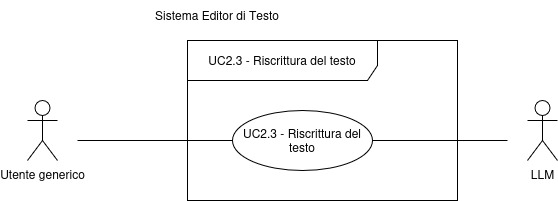
\includegraphics[width=0.8\textwidth]{../UCimg/UC2.3.jpg}
    \caption{Diagramma dei casi d'uso UC-2.3}
    \label{fig:uc2.3}
\end{figure}

\subsubsection{UC-2.4 - Traduzione del testo}
\begin{itemize}
    \item \textbf{Attore principale}: Utente generico
    \item \textbf{Descrizione}: Traduzione automatica del testo nella lingua selezionata
    \item \textbf{Precondizioni}: È presente testo nell’editor (completo o selezionato)
    \item \textbf{Postcondizioni}: La traduzione viene generata e inserita nell'editor, in seguito alla conferma dell'utente
    \item \textbf{Scenario principale}:
    \begin{itemize}
        \item L’utente seleziona la porzione di testo da tradurre (o nessuna selezione per l'intero documento)
        \item L’utente attiva il comando ”Traduci”
        \item L’utente definisce la lingua di destinazione
        \item Il sistema elabora la richiesta e invia il testo al LLM
        \item Il sistema mostra la traduzione generata
        \item L'utente conferma la proposta
        \item Il sistema inserisce il testo nell'editor
    \end{itemize}
    \item \textbf{Estensioni}:
    \begin{itemize}
        \item Il testo è già nella lingua selezionata: il testo originale rimane invariato e il sistema manda un messaggio all’utente
        \item L’utente non seleziona nessuna lingua di destinazione
    \end{itemize}
\end{itemize}

\subsubsection{UC-2.4.1 - Gestione mancata selezione della lingua di destinazione}
\begin{itemize}
    \item \textbf{Attore principale}: Utente generico
    \item \textbf{Descrizione}: L’utente attiva l’operazione di traduzione senza aver confermato una lingua di destinazione
    \item \textbf{Precondizioni}: È presente testo nell’editor (completo o selezionato) e l’utente attiva il comando di traduzione
    \item \textbf{Postcondizioni}: Viene generata la traduzione in inglese e viene inserita nel documento, in seguito alla conferma dell'utente
    \item \textbf{Scenario principale}:
    \begin{itemize}
        \item L’utente seleziona la porzione di testo da tradurre (o nessuna selezione per l'intero documento)
        \item L’utente attiva il comando ”Traduci” senza selezionare una lingua di destinazione
        \item Il sistema imposta la lingua inglese come lingua di default per la traduzione
        \item Il sistema elabora la richiesta e invia il testo al LLM
        \item Il sistema mostra la traduzione generata
        \item L'utente conferma la proposta
        \item Il sistema inserisce il testo nell'editor
    \end{itemize}
\end{itemize}

\begin{figure}[H]
    \centering
    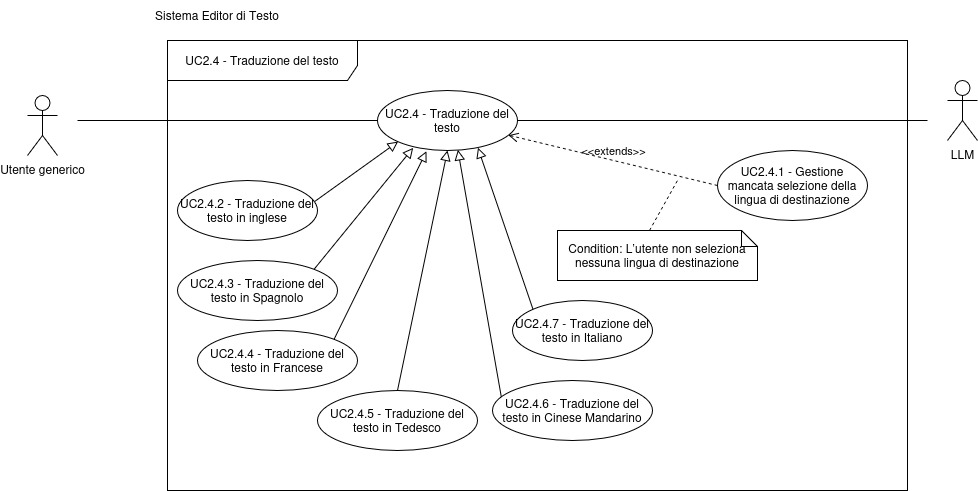
\includegraphics[width=0.8\textwidth]{../UCimg/UC2.4.jpg}
    \caption{Diagramma dei casi d'uso UC-2.4.*}
    \label{fig:uc2.4}
\end{figure}

\subsubsection{UC-2.4.2 - Traduzione del testo in Inglese}
\begin{itemize}
    \item \textbf{Attore principale}: Utente generico
    \item \textbf{Descrizione}: Traduzione automatica del testo nella lingua inglese
    \item \textbf{Precondizioni}: È presente testo nell’editor (completo o selezionato)
    \item \textbf{Postcondizioni}: Il testo viene tradotto in lingua inglese e inserito nel documento in seguito alla conferma dell'utente
    \item \textbf{Scenario principale}:
    \begin{itemize}
        \item L’utente seleziona la porzione di testo da tradurre (o nessuna selezione per l'intero documento)
        \item L’utente attiva il comando ”Traduci”
        \item L’utente imposta “Inglese” come lingua di destinazione
        \item Il sistema elabora la richiesta e invia il testo al LLM
        \item Il sistema mostra la traduzione generata
        \item L'utente conferma la proposta
        \item Il sistema inserisce il testo nell'editor
    \end{itemize}
\end{itemize}

\subsubsection{UC-2.4.3 - Traduzione del testo in Spagnolo}
\begin{itemize}
    \item \textbf{Attore principale}: Utente generico
    \item \textbf{Descrizione}: Traduzione automatica del testo nella lingua spagnola
    \item \textbf{Precondizioni}: È presente testo nell’editor (completo o selezionato)
    \item \textbf{Postcondizioni}: Il testo viene tradotto in lingua spagnola e inserito nel documento in seguito alla conferma dell'utente
    \item \textbf{Scenario principale}:
    \begin{itemize}
        \item L’utente seleziona la porzione di testo da tradurre (o nessuna selezione per l'intero documento)
        \item L’utente attiva il comando ”Traduci”
        \item L’utente imposta “Spagnolo” come lingua di destinazione
        \item Il sistema elabora la richiesta e invia il testo al LLM
        \item Il sistema mostra la traduzione generata
        \item L'utente conferma la proposta
        \item Il sistema inserisce il testo nell'editor
    \end{itemize}
\end{itemize}

\subsubsection{UC-2.4.4 - Traduzione del testo in Francese}
    \begin{itemize}
    \item \textbf{Attore principale}: Utente generico
    \item \textbf{Descrizione}: Traduzione automatica del testo nella lingua francese
    \item \textbf{Precondizioni}: È presente testo nell’editor (completo o selezionato)
    \item \textbf{Postcondizioni}: Il testo viene tradotto in lingua francese e inserito nel documento in seguito alla conferma dell'utente
    \item \textbf{Scenario principale}:
    \begin{itemize}
        \item L’utente seleziona la porzione di testo da tradurre (o nessuna selezione per l'intero documento)
        \item L’utente attiva il comando ”Traduci”
        \item L’utente imposta “Francese” come lingua di destinazione
        \item Il sistema elabora la richiesta e invia il testo al LLM
        \item Il sistema mostra la traduzione generata
        \item L'utente conferma la proposta
        \item Il sistema inserisce il testo nell'editor
    \end{itemize}
\end{itemize}

\subsubsection{UC-2.4.5 - Traduzione del testo in Tedesco}
\begin{itemize}
    \item \textbf{Attore principale}: Utente generico
    \item \textbf{Descrizione}: Traduzione automatica del testo nella lingua tedesca
    \item \textbf{Precondizioni}: È presente testo nell’editor (completo o selezionato)
    \item \textbf{Postcondizioni}: Il testo viene tradotto in lingua tedesca e inserito nel documento in seguito alla conferma dell'utente
    \item \textbf{Scenario principale}:
    \begin{itemize}
        \item L’utente seleziona la porzione di testo da tradurre (o nessuna selezione per l'intero documento)
        \item L’utente attiva il comando ”Traduci”
        \item L’utente imposta “Tedesco” come lingua di destinazione
        \item Il sistema elabora la richiesta e invia il testo al LLM
        \item Il sistema mostra la traduzione generata
        \item L'utente conferma la proposta
        \item Il sistema inserisce il testo nell'editor
    \end{itemize}
\end{itemize}

\subsubsection{UC-2.4.6 - Traduzione del testo in Cinese Mandarino}
\begin{itemize}
    \item \textbf{Attore principale}: Utente generico
    \item \textbf{Descrizione}: Traduzione automatica del testo nella lingua cinese mandarino
    \item \textbf{Precondizioni}: È presente testo nell’editor (completo o selezionato)
    \item \textbf{Postcondizioni}: Il testo viene tradotto in lingua cinese mandarino e inserito nel documento in seguito alla conferma dell'utente
    \item \textbf{Scenario principale}:
    \begin{itemize}
        \item L’utente seleziona la porzione di testo da tradurre (o nessuna selezione per l'intero documento)
        \item L’utente attiva il comando ”Traduci”
        \item L’utente imposta “Cinese Mandarino” come lingua di destinazione
        \item Il sistema elabora la richiesta e invia il testo al LLM
        \item Il sistema mostra la traduzione generata
        \item L'utente conferma la proposta
        \item Il sistema inserisce il testo nell'editor
    \end{itemize}
\end{itemize}

\subsubsection{UC-2.4.7 - Traduzione del testo in Italiano}
\begin{itemize}
    \item \textbf{Attore principale}: Utente generico
    \item \textbf{Descrizione}: Traduzione automatica del testo nella lingua Italiana
    \item \textbf{Precondizioni}: È presente testo nell’editor (completo o selezionato)
    \item \textbf{Postcondizioni}: Il testo viene tradotto in lingua Italiana e inserito nel documento in seguito alla conferma dell'utente
    \item \textbf{Scenario principale}:
    \begin{itemize}
        \item L’utente seleziona la porzione di testo da tradurre (o nessuna selezione per l'intero documento)
        \item L’utente attiva il comando ”Traduci”
        \item L’utente imposta “Italiano” come lingua di destinazione
        \item Il sistema elabora la richiesta e invia il testo al LLM
        \item Il sistema mostra la traduzione generata
        \item L'utente conferma la proposta
        \item Il sistema inserisce il testo nell'editor
    \end{itemize}
\end{itemize}

\subsubsection{UC-2.5 - Correzione grammaticale}
\begin{itemize}
    \item \textbf{Attore principale}: Utente generico
    \item \textbf{Descrizione}: Rilevamento e correzione automatica di errori grammaticali, ortografici e di punteggiatura
    \item \textbf{Precondizioni}: È presente testo nell’editor (completo o selezionato)
    \item \textbf{Postcondizioni}: Una versione corretta del testo viene inserita nell’editor in seguito alla conferma dell'utente
    \item \textbf{Scenario principale}:
    \begin{itemize}
        \item L’utente seleziona la porzione di testo da correggere (o nessuna selezione per l'intero documento)
        \item L’utente attiva il comando ”Correggi”
        \item Il sistema elabora la richiesta e invia il testo al LLM
        \item Il sistema rileva gli errori grammaticali e li mostra all'utente
        \item L'utente conferma le correzioni proposte
    \end{itemize}
    \item \textbf{Estensioni}:
    \begin{itemize}
        \item Non vengono rilevati errori
    \end{itemize}
\end{itemize}

\subsubsection{UC-2.5.1 - Nessun errore grammaticale rilevato}
\begin{itemize}
    \item \textbf{Attore principale}: Utente generico
    \item \textbf{Descrizione}: Dopo l’operazione di correzione grammaticale non vengono rilevati errori
    \item \textbf{Precondizioni}: È presente testo nell’editor (completo o selezionato) e l’utente ha attivato il comando di correzione grammaticale
    \item \textbf{Postcondizioni}: Non ci sono errori e il documento rimane invariato
    \item \textbf{Scenario principale}:
    \begin{itemize}
        \item Il sistema analizza il testo e non rileva errori
        \item Il sistema mostra una notifica all’utente
        \item Il testo originale rimane invariato e nessun nuovo blocco viene generato
    \end{itemize}
\end{itemize}

\begin{figure}[H]
    \centering
    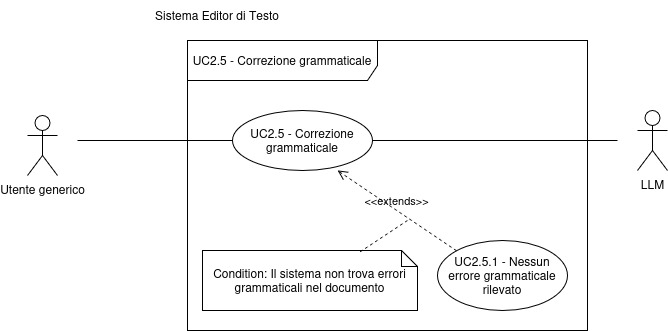
\includegraphics[width=0.8\textwidth]{../UCimg/UC2.5.jpg}
    \caption{Diagramma dei casi d'uso UC-2.5, 2.5.1}
    \label{fig:uc2.5}
\end{figure}

\subsubsection{UC-2.6 - Critica testuale con i 6 Cappelli di De Bono}
\begin{itemize}
    \item \textbf{Attore principale}: Utente generico
    \item \textbf{Descrizione}: Analisi del testo basata su una delle modalità del modello dei "Sei Cappelli per pensare" di Edward De Bono
    \item \textbf{Precondizioni}: È presente testo nell’editor (completo o selezionato)
    \item \textbf{Postcondizioni}: Viene generata un’analisi del testo secondo la prospettiva scelta e inserita nel documento in seguito alla conferma dell'utente
    \item \textbf{Scenario principale}:
    \begin{itemize}
        \item L’utente seleziona la porzione di testo da analizzare (o nessuna selezione per l'intero documento)
        \item L’utente attiva il menu ”Analisi critica”
        \item L’utente definisce la modalità di analisi (colore del Cappello) desiderata
        \item Il sistema elabora la richiesta e invia il testo al LLM
        \item Il sistema genera l'analisi 
        \item L'utente visualizza la critica generata
        \item L'utente può scegliere se inserire la critica generata nell'editor, rigenerarla o eliminarla
    \end{itemize}
    \item \textbf{Estensioni}:
    \begin{itemize}
        \item Il testo è troppo breve per un’analisi significativa
        \item L’utente non seleziona nessun colore per l’analisi
    \end{itemize}
\end{itemize}

\subsubsection{UC-2.6.1 - Gestione testo insufficiente per analisi critica}
\begin{itemize}
    \item \textbf{Attore principale}: Utente generico
    \item \textbf{Descrizione}: Gestione dell’errore nel caso in cui il contenuto selezionato non sia sufficiente per applicare il modello di analisi dei Sei Cappelli
    \item \textbf{Precondizioni}: È presente testo nell’editor e l’utente attiva il comando di analisi su una porzione di testo
    \item \textbf{Postcondizioni}: L’operazione viene annullata e viene mostrato un messaggio di avviso. Il testo originale rimane invariato
    \item \textbf{Scenario principale}:
    \begin{itemize}
        \item L’utente seleziona una porzione di testo molto breve da analizzare (o il documento contiene testo insufficiente)
        \item L’utente attiva il comando ”Analisi critica” e seleziona una modalità
        \item Il sistema rileva che la quantità di testo è inferiore alla soglia minima per produrre un'analisi semantica significativa
        \item Il sistema interrompe l'elaborazione
        \item Il sistema mostra un messaggio di avviso all'utente (es. "Testo troppo breve per l'analisi") suggerendo di aggiungere contenuto.
        \item Il testo originale rimane invariato e nessun blocco di analisi viene generato
    \end{itemize}
\end{itemize}

\subsubsection{UC-2.6.2 - Gestione mancata selezione della modalità di analisi}
\begin{itemize}
    \item \textbf{Attore principale}: Utente generico
    \item \textbf{Descrizione}: L’utente attiva l’analisi critica senza aver confermato uno specifico Cappello
    \item \textbf{Precondizioni}: È presente testo nell’editor e l’utente attiva il comando di analisi
    \item \textbf{Postcondizioni}: Viene generata un'analisi "Cappello Bianco" (default) inserita nel documento con formattazione distintiva
    \item \textbf{Scenario principale}:
    \begin{itemize}
        \item L’utente seleziona la porzione di testo da analizzare (o nessuna selezione per l'intero documento)
        \item L’utente attiva il comando ”Analisi critica” senza selezionare una modalità specifica
        \item Il sistema imposta il "Cappello Bianco" (Analisi Oggettiva) come modalità di default
        \item Il sistema elabora la richiesta e invia il testo al LLM
        \item L'utente visualizza l'analisi generata
    \end{itemize}
\end{itemize}

\begin{figure}[H]
    \centering
    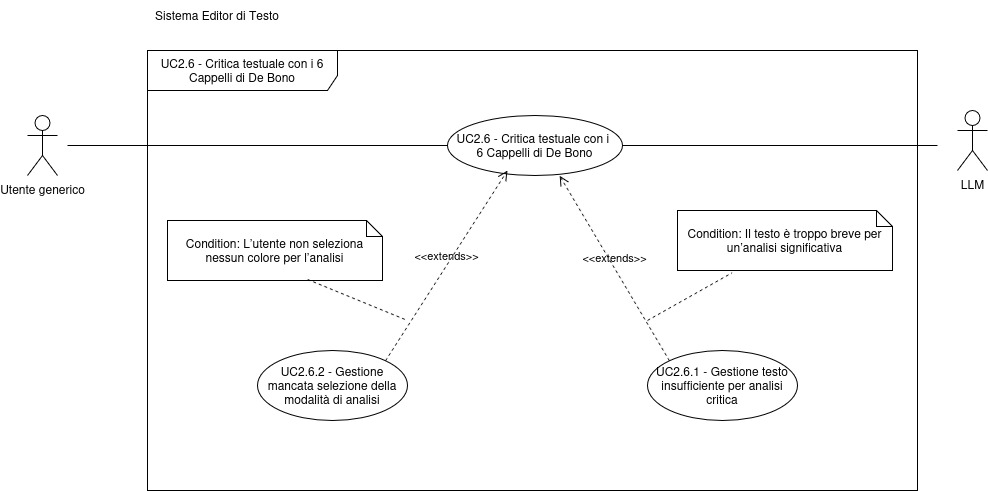
\includegraphics[width=0.8\textwidth]{../UCimg/UC2.6.jpg}
    \caption{Diagramma dei casi d'uso UC-2.6, 2.6.1, 2.6.2}
    \label{fig:uc2.6}
\end{figure}

\subsubsection{UC-2.6.3 - Critica testuale con il Cappello Bianco}
\begin{itemize}
    \item \textbf{Attore principale}: Utente generico
    \item \textbf{Descrizione}: Analisi oggettiva e fattuale del testo basata sul modello del Cappello Bianco di De Bono
    \item \textbf{Precondizioni}: È presente testo nell’editor
    \item \textbf{Postcondizioni}: Viene generata un’analisi fattuale inserita nel documento in seguito alla conferma dell'utente
    \item \textbf{Scenario principale}:
    \begin{itemize}
        \item L’utente seleziona il testo da analizzare (o nessuna selezione per l'intero documento)
        \item L’utente clicca sul menu ”Analisi critica”
        \item L’utente imposta ”Cappello Bianco” come modalità di analisi
        \item Il sistema elabora la richiesta e invia il testo al LLM
        \item Il sistema genera l'analisi 
        \item L'utente visualizza l'analisi generata
    \end{itemize}
\end{itemize}

\subsubsection{UC-2.6.4 - Critica testuale con il Cappello Rosso}
\begin{itemize}
    \item \textbf{Attore principale}: Utente generico
    \item \textbf{Descrizione}: Analisi emotiva e intuitiva del testo basata sul modello del Cappello Rosso di De Bono
    \item \textbf{Precondizioni}: È presente testo nell’editor
    \item \textbf{Postcondizioni}: Viene generata un’analisi emotiva inserita nel documento in seguito alla conferma dell'utente
    \item \textbf{Scenario principale}:
    \begin{itemize}
        \item L’utente seleziona il testo da analizzare (o nessuna selezione per l'intero documento)
        \item L’utente clicca sul menu ”Analisi critica”
        \item L’utente imposta ”Cappello Rosso” come modalità di analisi
        \item Il sistema elabora la richiesta e invia il testo al LLM
        \item Il sistema genera l'analisi 
        \item L'utente visualizza l'analisi generata
    \end{itemize}
\end{itemize}

\subsubsection{UC-2.6.5 - Critica testuale con il Cappello Nero}
\begin{itemize}
    \item \textbf{Attore principale}: Utente generico
    \item \textbf{Descrizione}: Analisi critica e cautelativa del testo basata sul modello del Cappello Nero di De Bono
    \item \textbf{Precondizioni}: È presente testo nell’editor
    \item \textbf{Postcondizioni}: Viene generata un’analisi critica inserita nel documento in seguito alla conferma dell'utente
    \item \textbf{Scenario principale}:
    \begin{itemize}
        \item L’utente seleziona il testo da analizzare (o nessuna selezione per l'intero documento)
        \item L’utente clicca sul menu ”Analisi critica”
        \item L’utente imposta ”Cappello Nero” come modalità di analisi
        \item Il sistema elabora la richiesta e invia il testo al LLM
        \item Il sistema genera l'analisi 
        \item L'utente visualizza l'analisi generata
    \end{itemize}
\end{itemize}

\subsubsection{UC-2.6.6 - Critica testuale con il Cappello Giallo}
\begin{itemize}
    \item \textbf{Attore principale}: Utente generico
    \item \textbf{Descrizione}: Analisi ottimistica e costruttiva del testo basata sul modello del Cappello Giallo di De Bono
    \item \textbf{Precondizioni}: È presente testo nell’editor
    \item \textbf{Postcondizioni}: Viene generata un’analisi ottimistica inserita nel documento in seguito alla conferma dell'utente
    \item \textbf{Scenario principale}:
    \begin{itemize}
        \item L’utente seleziona il testo da analizzare (o nessuna selezione per l'intero documento)
        \item L’utente clicca sul menu ”Analisi critica”
        \item L’utente imposta ”Cappello Giallo” come modalità di analisi
        \item Il sistema elabora la richiesta e invia il testo al LLM
        \item Il sistema genera l'analisi 
        \item L'utente visualizza l'analisi generata
    \end{itemize}
\end{itemize}

\subsubsection{UC-2.6.7 - Critica testuale con il Cappello Verde}
\begin{itemize}
    \item \textbf{Attore principale}: Utente generico
    \item \textbf{Descrizione}: Analisi creativa e innovativa del testo basata sul modello del Cappello Verde di De Bono
    \item \textbf{Precondizioni}: È presente testo nell’editor
    \item \textbf{Postcondizioni}: Viene generata un’analisi creativa inserita nel documento in seguito alla conferma dell'utente
    \item \textbf{Scenario principale}:
    \begin{itemize}
        \item L’utente seleziona il testo da analizzare (o nessuna selezione per l'intero documento)
        \item L’utente clicca sul menu ”Analisi critica”
        \item L’utente imposta ”Cappello Verde” come modalità di analisi
        \item Il sistema elabora la richiesta e invia il testo al LLM
        \item Il sistema genera l'analisi 
        \item L'utente visualizza l'analisi generata
    \end{itemize}
\end{itemize}

\subsubsection{UC-2.6.8 - Critica testuale con il Cappello Blu}
\begin{itemize}
    \item \textbf{Attore principale}: Utente generico
    \item \textbf{Descrizione}: Analisi processuale e organizzativa del testo basata sul modello del Cappello Blu di De Bono
    \item \textbf{Precondizioni}: È presente testo nell’editor
    \item \textbf{Postcondizioni}: Viene generata un’analisi processuale inserita nel documento in seguito alla conferma dell'utente
    \item \textbf{Scenario principale}:
    \begin{itemize}
        \item L’utente seleziona il testo da analizzare (o nessuna selezione per l'intero documento)
        \item L’utente clicca sul menu ”Analisi critica”
        \item L’utente imposta ”Cappello Blu” come modalità di analisi
        \item Il sistema elabora la richiesta e invia il testo al LLM
        \item Il sistema genera l'analisi 
        \item L'utente visualizza l'analisi generata
    \end{itemize}
\end{itemize}

\begin{figure}[H]
    \centering
    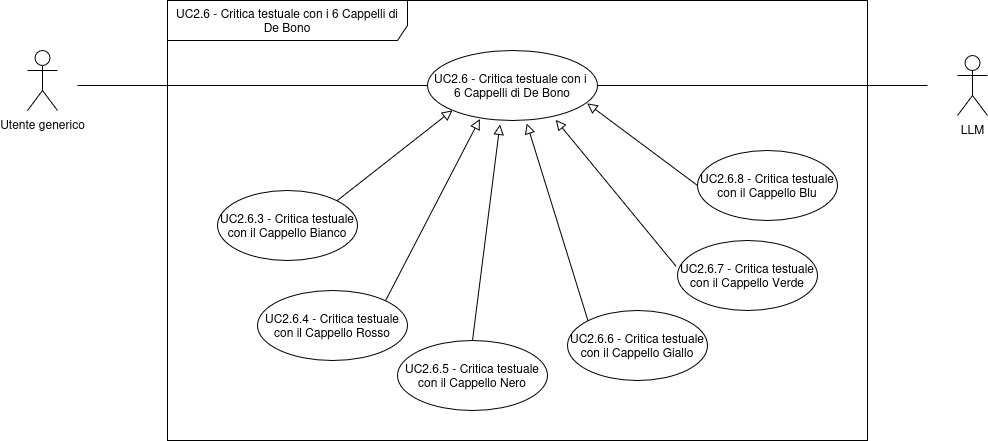
\includegraphics[width=0.8\textwidth]{../UCimg/UC2.6.3.jpg}
    \caption{Diagramma dei casi d'uso UC-2.6.3 - 2.6.8}
    \label{fig:uc2.6.3}
\end{figure}

\subsubsection{UC-2.7 - Generazione di testo (\gls{Distant Writing})}
\begin{itemize}
    \item \textbf{Attore principale}: Utente generico
    \item \textbf{Descrizione}: Creazione di nuovo testo inedito a partire da un \gls{prompt} descrittivo fornito dall’utente
    \item \textbf{Precondizioni}: L’editor è aperto e pronto per la scrittura
    \item \textbf{Postcondizioni}: Viene generato un nuovo testo basato sul \gls{prompt} e inserito nell’editor in seguito alla conferma dell'utente
    \item \textbf{Scenario principale}:
    \begin{itemize}
        \item L’utente si posiziona nel punto del documento dove vuole inserire il testo generato
        \item L’utente inserisce un \gls{prompt} descrivendo il contenuto desiderato (tramite chatbox o comando rapido)
        \item Il sistema invia il \gls{prompt} al LLM
        \item L'utente conferma la proposta
        \item Il sistema inserisce nell'editor il testo generato nel punto indicato
    \end{itemize}
    \item \textbf{Estensioni}:
    \begin{itemize}
        \item L’utente fornisce un \gls{prompt} troppo vago o incompleto
    \end{itemize}
\end{itemize}

\subsubsection{UC-2.7.1 - Gestione \gls{prompt} incompleto}
\begin{itemize}
    \item \textbf{Attore principale}: Utente generico
    \item \textbf{Descrizione}: Il sistema rileva una richiesta poco chiara o incompleta e guida l'utente nel miglioramento del \gls{prompt} prima di invocare l'AI
    \item \textbf{Precondizioni}: L'utente ha avviato una richiesta di generazione testo (\gls{Distant Writing})
    \item \textbf{Postcondizioni}: La generazione viene sospesa e all'utente vengono forniti suggerimenti operativi per affinare la richiesta
    \item \textbf{Scenario principale}:
    \begin{itemize}
        \item L’utente si posiziona nel punto del documento dove vuole inserire il testo generato
        \item L’utente inserisce un \gls{prompt} descrivendo il contenuto desiderato (tramite chatbox o comando rapido)
        \item LLM analizza il \gls{prompt} e lo valuta come troppo vago, breve o privo di contesto sufficiente
        \item Il sistema interrompe la richiesta e mostra un messaggio di avviso chiedendo chiarimenti
        \item Il sistema propone esempi di \gls{prompt} efficaci o template basati sul contesto corrente (opzionale)
        \item Il sistema rimane in attesa di un nuovo input migliorativo da parte dell'utente
    \end{itemize}
\end{itemize}

\begin{figure}[H]
    \centering
    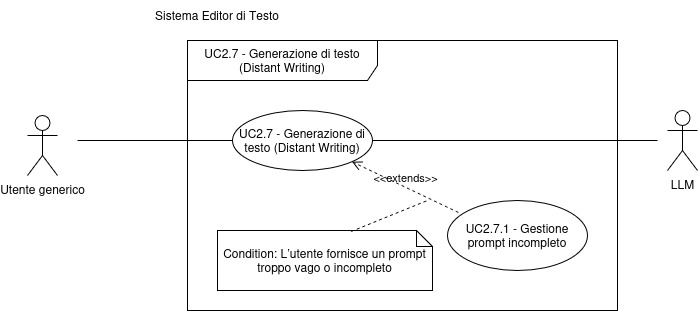
\includegraphics[width=0.8\textwidth]{../UCimg/UC2.7.jpg}
    \caption{Diagramma dei casi d'uso UC-2.7, 2.7.1}
    \label{fig:uc2.7}
\end{figure}

\subsubsection{UC-2.8 - Generazione di grafici e tabelle}
\begin{itemize}
    \item \textbf{Attore principale}: Utente generico
    \item \textbf{Descrizione}: Creazione automatica di appresentazioni visive basate su dati descritti nel testo. I tipi di visualizzazione supportati sono:
        \begin{itemize}
            \item Tabella
            \item Grafico a barre
            \item Grafico a torta
            \item Grafico a linee
        \end{itemize}
    \item \textbf{Precondizioni}: È presente testo descrittivo contenente dati nell’editor
    \item \textbf{Postcondizioni}: Viene generato un elemento grafico o tabellare inserito nel documento in seguito alla conferma dell'utente
    \item \textbf{Scenario principale}:
    \begin{itemize}
    \item L’utente seleziona la porzione di testo contenente i dati
    \item L’utente attiva il comando ”Genera grafico/tabella”
    \item L’utente specifica il tipo di visualizzazione desiderata (tabella, grafico a barre, a torta, a linee)
    \item Il sistema elabora la richiesta e invia i dati al LLM
    \item Il sistema genera l'elemento visivo 
    \item L'utente conferma la proposta 
    \item Il sistema inserisce l'elemento visivo nell'editor, dopo il testo selezionato
    \end{itemize}
    \item \textbf{Estensioni}:
    \begin{itemize}
        \item Il testo non contiene dati strutturati sufficienti
    \end{itemize}
\end{itemize}

\subsubsection{UC-2.8.1 - Gestire dati insufficienti per la visualizzazione di grafici e tabelle}
\begin{itemize}
    \item \textbf{Attore principale}: Utente generico
    \item \textbf{Descrizione}: Il sistema rileva l'impossibilità di creare un grafico o una tabella a causa della mancanza di dati strutturati nel testo selezionato
    \item \textbf{Precondizioni}: L’utente ha attivato il comando di generazione grafico/tabella su una selezione di testo
    \item \textbf{Postcondizioni}: L’operazione viene annullata e viene mostrato un messaggio di avviso. Il testo originale rimane invariato
    \item \textbf{Scenario principale}:
    \begin{itemize}
        \item L'utente attiva il comando "Genera grafico/tabella" su una porzione di testo
        \item Il sistema elabora la richiesta e invia i dati al LLM
        \item LLM analizza il contenuto selezionato per estrarre serie di dati
        \item LLM rileva che il testo è puramente descrittivo o privo di valori numerici/categorici sufficienti per una rappresentazione visiva
        \item Il sistema interrompe la generazione dell'elemento visivo
        \item Il sistema mostra un avviso all'utente
        \item Il testo originale rimane invariato
    \end{itemize}
\end{itemize}

\begin{figure}[H]
    \centering
    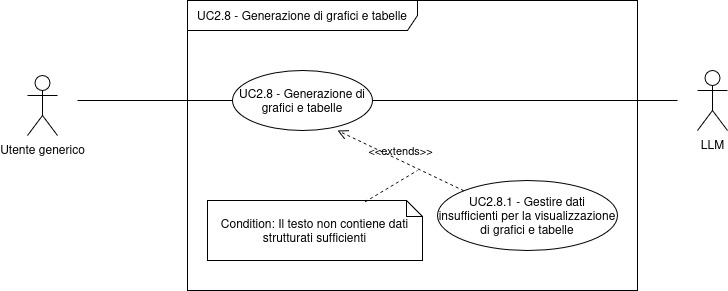
\includegraphics[width=0.8\textwidth]{../UCimg/UC2.8.jpg}
    \caption{Diagramma dei casi d'uso UC-2.8, 2.8.1}
    \label{fig:uc2.8}
\end{figure}

\subsubsection{UC-2.9 - Generazione di mappe concettuali}
\begin{itemize}
    \item \textbf{Attore principale}: Utente generico
    \item \textbf{Descrizione}: Creazione automatica di mappe concettuali per visualizzare le relazioni logiche tra i concetti presenti nel testo
    \item \textbf{Precondizioni}: È presente testo nell’editor (completo o selezionato)
    \item \textbf{Postcondizioni}: Viene generata una mappa concettuale che viene inserita nel documento
    \item \textbf{Scenario principale}:
    \begin{itemize}
        \item L’utente seleziona il testo da visualizzare come mappa (o nessuna selezione per l'intero documento)
        \item L’utente attiva il comando ”Genera mappa concettuale”
        \item Il sistema elabora la richiesta e invia il testo al LLM
        \item Il sistema renderizza la mappa concettuale
        \item L'utente conferma la proposta 
        \item Il sistema inserisce la mappa nell'editor, applicando lo stile distintivo per il contenuto generato
    \end{itemize}
    \item \textbf{Estensioni}:
    \begin{itemize}
        \item Errore di visualizzazione o generazione della mappa
    \end{itemize}
\end{itemize}

\subsubsection{UC-2.9.1 - Gestione errori di visualizzazione delle mappe concettuali generate}
\begin{itemize}
    \item \textbf{Attore principale}: Utente generico
    \item \textbf{Descrizione}: Il sistema gestisce il fallimento del rendering grafico della mappa concettuale fornendo il codice sorgente utilizzabile esternamente
    \item \textbf{Precondizioni}: L’utente ha attivato la generazione di una mappa concettuale
    \item \textbf{Postcondizioni}: Il codice sorgente della mappa viene inserito nel documento al posto della rappresentazione grafica
    \item \textbf{Scenario principale}:
    \begin{itemize}
        \item Il sistema tenta di renderizzare la mappa concettuale generata dal LLM
        \item Il sistema rileva un errore di visualizzazione o una incompatibilità tecnica
        \item Il sistema mostra un avviso all'utente
        \item Il sistema inserisce nel documento il blocco di codice sorgente eseguibile (es. sintassi Mermaid o Graphviz) generato dal LLM, permettendo all'utente di generarla con strumenti esterni
    \end{itemize}
\end{itemize}

\begin{figure}[H]
    \centering
    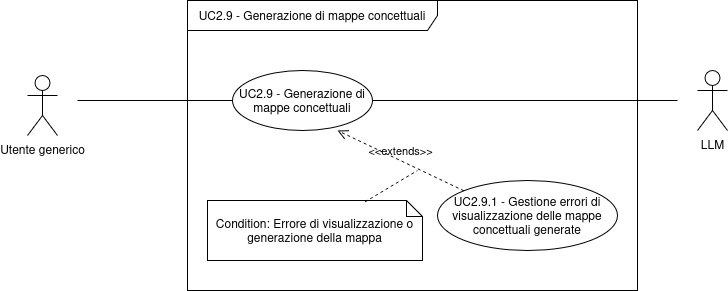
\includegraphics[width=0.8\textwidth]{../UCimg/UC2.9.jpg}
    \caption{Diagramma dei casi d'uso UC-2.9, 2.9.1}
    \label{fig:uc2.9}
\end{figure}

\subsubsection{UC-2.10 - Generazione di formule matematiche}
\begin{itemize}
    \item \textbf{Attore principale}: Utente generico
    \item \textbf{Descrizione}: Conversione automatica di descrizioni testuali di problemi matematici in formule formattate
    \item \textbf{Precondizioni}: È presente testo descrittivo di un problema matematico nell’editor
    \item \textbf{Postcondizioni}: Vengono generate le formule matematiche corrispondenti e inserite nel documento con formattazione distintiva
    \item \textbf{Scenario principale}:
    \begin{itemize}
    \item L’utente seleziona il testo descrittivo del problema
    \item L’utente attiva il comando ”Genera formule”
    \item Il sistema elabora la richiesta e invia il testo al LLM
    \item Il sistema genera il codice matematico (simile LaTeX) 
    \item L'utente conferma la proposta
    \item Il sistema inserisce la formula nell'editor renderizzandolo
    \end{itemize}
    \item \textbf{Estensioni}:
    \begin{itemize}
        \item Il sistema non supporta simboli matematici complessi
    \end{itemize}
\end{itemize}

\subsubsection{UC-2.10.1 - Gestire simboli non supportati}
\begin{itemize}
    \item \textbf{Attore principale}: Utente generico
    \item \textbf{Descrizione}: Il sistema gestisce la presenza di notazioni matematiche complesse non supportate dal motore di rendering locale
    \item \textbf{Precondizioni}: L’utente ha attivato la generazione di formule matematiche
    \item \textbf{Postcondizioni}: La formula viene inserita come codice grezzo o testo approssimato invece che renderizzata graficamente
    \item \textbf{Scenario principale}:
    \begin{itemize}
        \item Il sistema analizza l'output matematico generato dal LLM
        \item Il sistema identifica simboli o costrutti non supportati dal motore di rendering integrato
        \item Il sistema segnala la limitazione all'utente tramite un avviso
        \item Il sistema inserisce la formula in formato codice grezzo o in una rappresentazione testuale approssimata, applicando lo stile distintivo per il contenuto generato
    \end{itemize}
\end{itemize}

\begin{figure}[H]
    \centering
    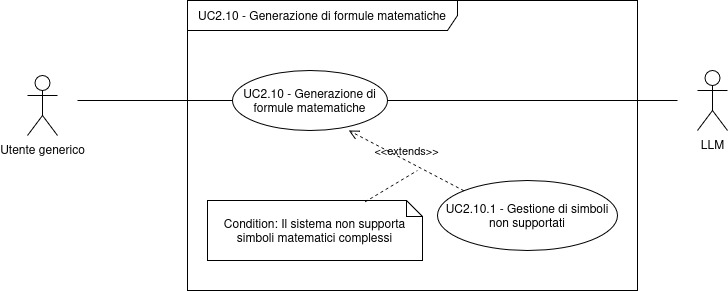
\includegraphics[width=0.8\textwidth]{../UCimg/UC2.10.jpg}
    \caption{Diagramma dei casi d'uso UC-2.10, 2.10.1}
    \label{fig:uc2.10}
\end{figure}

\newpage

\subsection{Macroarea 3 - Persistenza: Caricamento}
\subsubsection{UC-3.0 - Caricamento file}
\begin{itemize}
    \item \textbf{Attore principale}: Utente generico
    \item \textbf{Descrizione}: Permettere all'utente di caricare un documento nell'editor
    \item \textbf{Precondizioni}: L'utente ha un file che vuole caricare nell'editor
    \item \textbf{Postcondizioni}: L'utente ha caricato con successo il file nell'editor
    \item \textbf{Scenario principale}:
        \begin{itemize}
            \item Utente vuole caricare un file
            \item Utente clicca il pulsante per caricare il file
            \item Utente sceglie tra due opzioni: trascina file e esplora file
            \item Utente carica il documento
        \end{itemize}
    \item \textbf{Estensioni}:
        \begin{itemize}
            \item Utente seleziona un file non supportato
            \item Utente seleziona un file troppo grande
        \end{itemize}
\end{itemize}

\subsubsection{UC-3.0.1 - Caricamento file \gls{Markdown}}
\begin{itemize}
    \item \textbf{Attore principale}: Utente generico
    \item \textbf{Descrizione}: L'utente carica un file in formato \gls{Markdown} (\texttt{.md}, \texttt{.\gls{markdown}}) nell'editor
    \item \textbf{Precondizioni}: L'utente dispone di un file in formato \gls{Markdown}
    \item \textbf{Postcondizioni}: Il contenuto del file \gls{Markdown} viene caricato nell'editor
    \item \textbf{Scenario principale}:
        \begin{itemize}
            \item L'utente seleziona un file con estensione \texttt{.md} o \texttt{.\gls{markdown}}
            \item Il sistema carica il contenuto del file nell'editor
        \end{itemize}
\end{itemize}

\subsubsection{UC-3.0.2 - Caricamento file di testo}
\begin{itemize}
    \item \textbf{Attore principale}: Utente generico
    \item \textbf{Descrizione}: L'utente carica un file in formato testo semplice (\texttt{.txt}) nell'editor
    \item \textbf{Precondizioni}: L'utente dispone di un file in formato \texttt{.txt}
    \item \textbf{Postcondizioni}: Il contenuto del file di testo viene caricato nell'editor
    \item \textbf{Scenario principale}:
        \begin{itemize}
            \item L'utente seleziona un file con estensione \texttt{.txt}
            \item Il sistema carica il contenuto del file nell'editor
        \end{itemize}
\end{itemize}

\begin{figure}[H]
    \centering
    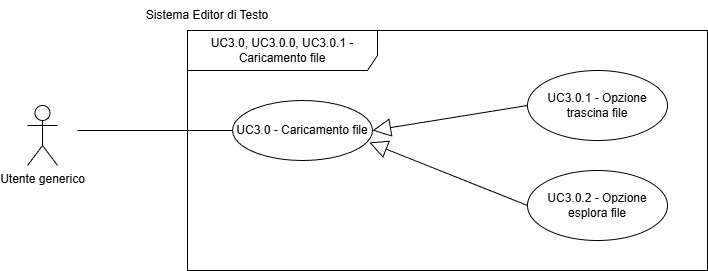
\includegraphics[width=0.8\textwidth]{../UCimg/UC3.0.jpg}
    \caption{Diagramma dei casi d'uso UC-3.0, 3.0.1, 3.0.2}
    \label{fig:uc3.0}
\end{figure}


\subsubsection{UC-3.0.3 - Caricamento tramite trascinamento (drag-and-drop)}
\begin{itemize}
    \item \textbf{Attore principale}: Utente generico
    \item \textbf{Descrizione}: L'utente carica un file nell'editor trascinandolo direttamente nell'area di editing, senza aprire il dialogo di esplorazione file
    \item \textbf{Precondizioni}:L'editor è aperto e l'utente dispone di un file da caricare
    \item \textbf{Postcondizioni}: Il contenuto del file trascinato viene caricato nell'editor
    \item \textbf{Scenario principale}:
        \begin{itemize}
            \item L'utente trascina un file dal proprio filesystem nell'area dell'editor
            \item Il sistema intercetta l'evento di rilascio del file (drop)
            \item Il sistema \gls{verifica} il formato e le dimensioni del file
            \item Il sistema carica il contenuto del file nell'editor
        \end{itemize}
\end{itemize}

\subsubsection{UC-3.0.4 - Caricamento tramite dialogo di esplorazione file (file picker)}
\begin{itemize}
    \item \textbf{Attore principale}: Utente generico
    \item \textbf{Descrizione}: L'utente carica un file nell'editor selezionandolo tramite il dialogo nativo del browser per l'esplorazione del filesystem
    \item \textbf{Precondizioni}: L'utente ha attivato il comando di caricamento file
    \item \textbf{Postcondizioni}: Il file selezionato tramite il dialogo viene passato al sistema per il caricamento nell'editor
    \item \textbf{Scenario principale}:
        \begin{itemize}
            \item Il sistema apre il dialogo nativo del browser per la selezione di file
            \item L'utente naviga nel proprio filesystem e seleziona il file desiderato
            \item L'utente conferma la selezione
            \item Il file selezionato viene restituito al sistema per il caricamento
        \end{itemize}
    \item \textbf{Estensioni}:
    \begin{itemize}
        \item L'utente chiude il dialogo senza selezionare alcun file: l'operazione viene annullata e l'editor rimane invariato
    \end{itemize}
\end{itemize}

\begin{figure}[H]
    \centering
    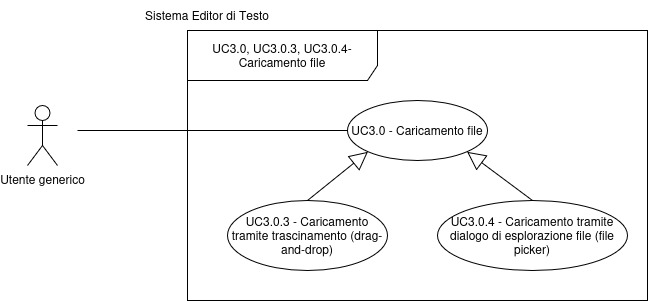
\includegraphics[width=0.8\textwidth]{../UCimg/UC3.0.3.jpg}
    \caption{Diagramma dei casi d'uso UC-3.0, 3.0.3, 3.0.4}
    \label{fig:uc3.0.3}
\end{figure}

\subsubsection{UC-3.1 - Gestione formati file non supportati}
\begin{itemize}
    \item \textbf{Attore principale}: Utente generico
    \item \textbf{Descrizione}: L'utente prova a caricare un documento ma è di un formato non supportato
    \item \textbf{Precondizioni}: Il file caricato è di un formato non supportato
    \item \textbf{Postcondizioni}: Appare il messaggio di errore "Formato non supportato"
    \item \textbf{Scenario principale}:
        \begin{itemize}
            \item L'utente seleziona un file tramite "Esplora file" o lo trascina nell'area di caricamento
            \item Il sistema analizza il tipo del file selezionato
            \item Il sistema rileva che il formato non è tra quelli supportati
            \item Il sistema blocca il processo di caricamento
            \item Viene visualizzato a schermo un messaggio di errore
        \end{itemize}
\end{itemize}

\subsubsection{UC-3.2 - Gestione file troppo grandi}
\begin{itemize}
    \item \textbf{Attore principale}: Utente generico
    \item \textbf{Descrizione}: L'utente prova a caricare un documento ma è di dimensioni troppo grandi
    \item \textbf{Precondizioni}: Il file caricato è di dimensioni troppo grandi
    \item \textbf{Postcondizioni}: Appare il messaggio di errore "File troppo grande"
    \item \textbf{Scenario principale}:
        \begin{itemize}
            \item L'utente seleziona un file tramite "Esplora file" o lo trascina nell'area di caricamento
            \item Il sistema controlla la dimensione del file
            \item Il sistema rileva che la dimensione del file supera il limite massimo consentito
            \item Il sistema blocca il processo di caricamento
            \item Viene visualizzato a schermo un messaggio di errore
        \end{itemize}
\end{itemize}

\subsubsection{UC-3.3 - Rimozione file caricato}
\begin{itemize}
    \item \textbf{Attore principale}: Utente generico
    \item \textbf{Descrizione}: utente vuole rimuovere un file che ha caricato
    \item \textbf{Precondizioni}: utente clicca tasto per rimuovere file caricato
    \item \textbf{Postcondizioni}: utente ha rimosso con successo il file
    \item \textbf{Scenario principale}:
        \begin{itemize}
            \item Utente clicca il pulsante rimuovi file
            \item Utente vede la schermata “Sei sicuro di voler rimuovere?”
            \item Utente preme si e rimuove con successo il file
        \end{itemize}
        \item \textbf{Estensioni}:
        \begin{itemize}
            \item Utente clicca no nella schermata “Sei sicuro di voler rimuovere?” e quindi il file non viene rimosso
        \end{itemize}
\end{itemize}

\subsubsection{UC-3.3.1 - Annullamento rimozione file caricato}
\begin{itemize}
    \item \textbf{Attore principale}: Utente generico
    \item \textbf{Descrizione}: utente annulla la rimozione di un file che ha caricato
    \item \textbf{Precondizioni}: utente clicca tasto tasto no nella schermata "Sei sicuro di voler rimuovere?"
    \item \textbf{Postcondizioni}: il file non viene rimosso
    \item \textbf{Scenario principale}:
        \begin{itemize}
            \item Utente clicca l'opzione no nella schermata "Sei sicuro di voler rimuovere?"
            \item La rimozione del file viene annullata
            \item L'utente torna nella pagina del file che ha caricato
        \end{itemize}
\end{itemize}

\begin{figure}[H]
    \centering
    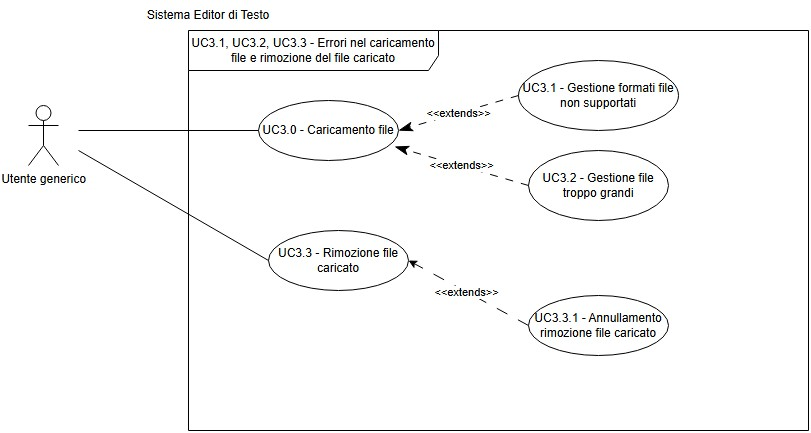
\includegraphics[width=0.8\textwidth]{../UCimg/UC3.1_3.2_3.jpg}
    \caption{Diagramma dei casi d'uso UC-3.1, 3.2, 3.3}
    \label{fig:uc3.1}
\end{figure}

\newpage

\subsection{Macroarea 4 - Persistenza: Salvataggio}
\subsubsection{UC-4.0 - Esportazione di un file}
\begin{itemize}
    \item \textbf{Attore principale}: Utente generico
    \item \textbf{Descrizione}: L'utente esporta il documento corrente in un formato a scelta tra quelli supportati dal sistema. Di default viene esportato l'intero documento; l'utente può opzionalmente limitare l'esportazione a pagine selezionate o a un intervallo
    \item \textbf{Precondizioni}: È presente testo nell'editor
    \item \textbf{Postcondizioni}: Il documento viene convertito nel formato selezionato e salvato localmente sul dispositivo dell'utente
    \item \textbf{Scenario principale}:
        \begin{itemize}
            \item L'utente attiva il comando di esportazione
            \item Il sistema presenta le opzioni di formato disponibili
            \item L'utente seleziona il formato desiderato
            \item Il sistema converte il documento nel formato selezionato
            \item Il sistema avvia il download del file sul dispositivo dell'utente
        \end{itemize}
\end{itemize}

\subsubsection{UC-4.0.1 - Esportare un file in PDF}
\begin{itemize}
    \item \textbf{Attore principale}: Utente generico
    \item \textbf{Descrizione}: Testo compilato salvato in locale sulla propria macchina in formato PDF
    \item \textbf{Precondizioni}: L'utente ha un documento che desidera scaricare
    \item \textbf{Postcondizioni}: L'utente ottiene un documento in formato PDF salvato localmente
    \item \textbf{Scenario principale}:
        \begin{itemize}
            \item Utente seleziona l'opzione "PDF" tra le opzioni di esportazione
            \item Il documento viene convertito in formato PDF
            \item Utente ottiene il documento salvato in PDF
        \end{itemize}
\end{itemize}

\subsubsection{UC-4.0.2 - Esportare un file in MD}
\begin{itemize}
    \item \textbf{Attore principale}: Utente generico
    \item \textbf{Descrizione}: Testo compilato salvato in locale sulla propria macchina in formato testuale
    \item \textbf{Precondizioni}: L'utente ha un documento che desidera scaricare
    \item \textbf{Postcondizioni}: L'utente ottiene un documento in formato MD salvato localmente
    \item \textbf{Scenario principale}:
        \begin{itemize}
            \item Utente seleziona opzione "src" tra le opzioni di esportazione
            \item Il documento viene salvato in formato MD
        \end{itemize}
\end{itemize}

\subsubsection{UC-4.0.3 - Esportare un file in formato HTML}
\begin{itemize}
    \item \textbf{Attore principale}: Utente generico
    \item \textbf{Descrizione}: Genera del codice HTML dal testo \gls{Markdown}
    \item \textbf{Precondizioni}: L'utente ha un documento non vuoto
    \item \textbf{Postcondizioni}: L'utente ottiene un file .HTML in cui viene convertito il testo \gls{Markdown} in codice HTML
    \item \textbf{Scenario principale}:
        \begin{itemize}
            \item Utente seleziona opzione "HTML" tra le opzioni di esportazione
            \item Il documento viene convertito in formato HTML
            \item Utente riceve il documento in formato HTML
        \end{itemize}
\end{itemize}

\subsubsection{UC-4.0.4 - Esportare un file in formato ODT}
\begin{itemize}
    \item \textbf{Attore principale}: Utente generico
    \item \textbf{Descrizione}: Genera documenti compatibili con popolari editor testuali
    \item \textbf{Precondizioni}: L'utente ha un documento non vuoto
    \item \textbf{Postcondizioni}: L'utente ottiene un file .ODT salvato localmente
    \item \textbf{Scenario principale}:
        \begin{itemize}
            \item Utente seleziona opzione "ODT" tra le opzioni di esportazione
            \item Il documento viene convertito in formato ODT
            \item Utente riceve il documento in formato ODT
        \end{itemize}
\end{itemize}

\subsubsection{UC-4.0.5 - Esportare un file in formato DOCX}
\begin{itemize}
    \item \textbf{Attore principale}: Utente generico
    \item \textbf{Descrizione}: Genera documenti compatibili con Microsoft Word
    \item \textbf{Precondizioni}: L'utente ha un documento non vuoto
    \item \textbf{Postcondizioni}: L'utente ottiene un file .DOCX salvato localmente
    \item \textbf{Scenario principale}:
        \begin{itemize}
            \item Utente seleziona opzione "DOCX" tra le opzioni di esportazione
            \item Il documento viene convertito in formato DOCX
            \item Utente riceve il documento in formato DOCX
        \end{itemize}
\end{itemize}
\begin{figure}[H]
    \centering
    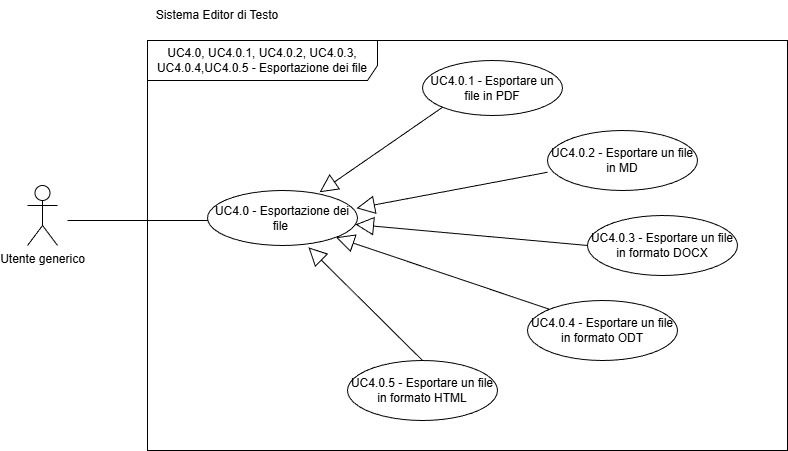
\includegraphics[width=0.8\textwidth]{../UCimg/UC4.0.jpg}
    \caption{Diagramma dei casi d'uso UC-4.0, UC-4.0.1, UC-4.0.2, UC-4.0.3, UC-4.0.4, UC-4.0.5*}
    \label{fig:uc4.0}
\end{figure}

\subsubsection{UC-4.0.6 - Esportare selezionate pagine del documento}
\begin{itemize}
    \item \textbf{Attore principale}: Utente generico
    \item \textbf{Descrizione}: Scaricare nel formato desiderato solo alcune pagine del documento
    \item \textbf{Precondizioni}: L'utente ha un documento non vuoto, con diverse pagine
    \item \textbf{Postcondizioni}: L'utente ottiene un file in formato a scelta con solo le pagine selezionate
    \item \textbf{Scenario principale}:
        \begin{itemize}
            \item Utente vuole scaricare solo selezionate pagine del documento da salvare
            \item Tra le opzioni di esportazione, elenca numericamente le pagine desiderate
            \item Seleziona modalità di esportazione
            \item Ottiene le pagine selezionate in un nuovo documento, salvato nel formato selezionato
        \end{itemize}
\end{itemize}

\subsubsection{UC-4.0.7 - Esportare un range di pagine del documento}
\begin{itemize}
    \item \textbf{Attore principale}: Utente generico
    \item \textbf{Descrizione}: Scaricare nel formato desiderato solo un range di pagine del documento
    \item \textbf{Precondizioni}: L'utente ha un documento non vuoto, con diverse pagine
    \item \textbf{Postcondizioni}: L'utente ottiene un file in formato a scelta con solo il range di pagine selezionate
    \item \textbf{Scenario principale}:
        \begin{itemize}
            \item Utente vuole scaricare porzioni consecutive di un documento
            \item Utente seleziona la pagina di inizio e fine del range da scaricare
            \item Seleziona modalità di esportazione
            \item Ottiene le pagine selezionate in un nuovo documento, salvato nel formato selezionato
        \end{itemize}
\end{itemize}
\begin{figure}[H]
    \centering
    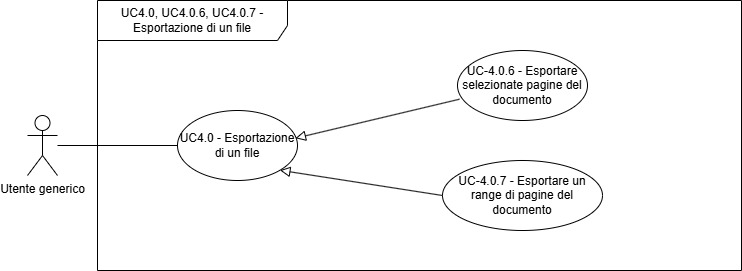
\includegraphics[width=0.8\textwidth]{../UCimg/UC4.0.6.jpg}
    \caption{Diagramma dei casi d'uso UC-4.0, UC-4.0.6, UC-4.0.7}
    \label{fig:uc4.0.6}
\end{figure}

\subsubsection{UC-4.1 - Stampare il documento}
\begin{itemize}
    \item \textbf{Attore principale}: Utente generico
    \item \textbf{Descrizione}: Utente desidera stampare il documento senza doverlo prima esportare
    \item \textbf{Precondizioni}: L'utente ha un documento aperto
    \item \textbf{Postcondizioni}: L'utente ottiene il documento stampato
    \item \textbf{Scenario principale}:
        \begin{itemize}
            \item Utente ha un documento aperto che desidera stampare
            \item Utente preme un pulsante "stampa"
            \item Utente ha accesso alle opzioni di stampa offerte dal suo browser
            \item Utente ritorna al proprio documento una volta completata l'operazione
        \end{itemize}
    \item \textbf{Estensioni}:
        \begin{itemize}
            \item L'utente stampa solo selezionate pagine del documento
        \end{itemize}
\end{itemize}

\begin{figure}[H]
    \centering
    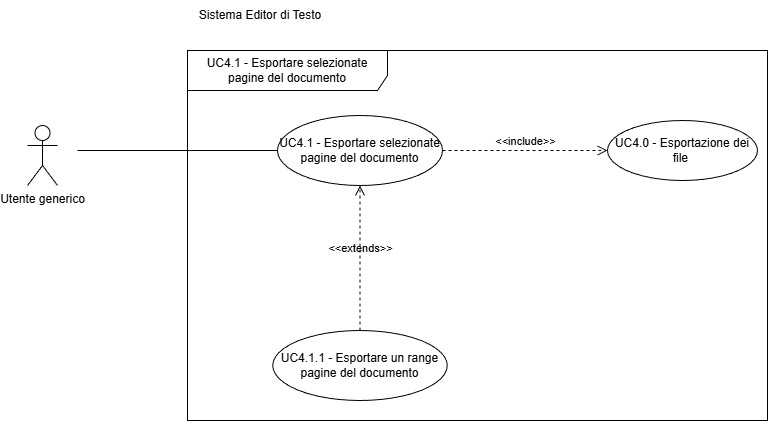
\includegraphics[width=0.8\textwidth]{../UCimg/UC4.1.jpg}
    \caption{Diagramma dei casi d'uso UC-4.1}
    \label{fig:uc4.1}
\end{figure}

\subsubsection{UC-4.2 - Apertura di un file salvato}
\begin{itemize}
    \item \textbf{Attore principale}: \gls{Utente autenticato}
    \item \textbf{Descrizione}: L'\gls{utente autenticato} può aprire un documento precedentemente salvato nel proprio account
    \item \textbf{Precondizioni}: L'utente è autenticato nel sistema e ha almeno un documento salvato nel proprio account
    \item \textbf{Postcondizioni}: Il documento selezionato viene caricato 
    nell'editor e l'utente può riprendere a modificarlo
    \item \textbf{Scenario principale}:
        \begin{itemize}
            \item L'utente accede all'area personale, dove può visualizzare i documenti salvati
            \item Il sistema mostra i documenti salvati dall'\gls{utente autenticato}
            \item L'utente seleziona il file da aprire
            \item Il sistema carica il contenuto del documento nell'editor
            \item L'utente può riprendere la modifica del documento
        \end{itemize}
    \item \textbf{Estensioni}:
        \begin{itemize}
            \item L'utente seleziona "annulla" nel pop up di selezione
        \end{itemize}
\end{itemize}

\subsubsection{UC-4.2.1 - Gestione annullamento apertura}
\begin{itemize}
    \item \textbf{Attore principale}: \gls{Utente autenticato}
    \item \textbf{Descrizione}: Il sistema gestisce l'interruzione della procedura di apertura file senza effettuare caricamenti
    \item \textbf{Precondizioni}: La finestra di selezione dei file è aperta
    \item \textbf{Postcondizioni}: La finestra viene chiusa e l'editor mantiene lo stato precedente (nessun file caricato o file precedente mantenuto)
    \item \textbf{Scenario principale}:
    \begin{itemize}
        \item L’utente, all'interno della finestra di selezione, clicca sul pulsante ”Annulla” (o chiude il popup)
        \item Il sistema chiude la finestra di dialogo
        \item Il sistema abortisce l'operazione di recupero dati dal \gls{database}
        \item L'interfaccia dell'editor rimane invariata rispetto allo stato precedente l'apertura della finestra
    \end{itemize}
\end{itemize}

\begin{figure}[H]
    \centering
    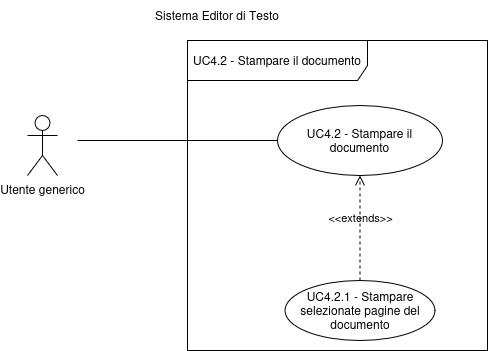
\includegraphics[width=0.8\textwidth]{../UCimg/UC4.2.jpg}
    \caption{Diagramma dei casi d'uso UC-4.2, 4.2.1}
    \label{fig:uc4.2}
\end{figure}

\subsubsection{UC-4.3 - Salvataggio file nel \gls{DataBase}}
\begin{itemize}
    \item \textbf{Attore principale}: \gls{Utente autenticato}
    \item \textbf{Descrizione}: L'utente vuole salvare la nota scritta nel \gls{database}, senza scaricarla nel suo dispositivo corrente
    \item \textbf{Precondizioni}: L'utente ha scritto una nota ed ha eseguito l'accesso al sistema con il suo account
    \item \textbf{Postcondizioni}: Il sistema mantiene nel \gls{Database} una copia della nota scritta, legandola all'account dell'utente
    \item \textbf{Scenario principale}:
        \begin{itemize}
            \item L'utente accede al sistema
            \item L'utente scrive del testo o ne genera con l'opzione relativa
            \item L'utente seleziona l'opzione di salvataggio
            \item Il sistema salva nel db una copia della nota dell'utente
        \end{itemize}
    \item \textbf{Estensioni}:
        \begin{itemize}
            \item L'utente non ha scritto o generato alcun testo
            \item L'utente non è autenticato
        \end{itemize}
\end{itemize}

\subsubsection{UC-4.3.1 - Gestione tentativo salvataggio nota vuota}
\begin{itemize}
    \item \textbf{Attore principale}: \gls{Utente autenticato}
    \item \textbf{Descrizione}: Il sistema impedisce il salvataggio di documenti privi di contenuto nel \gls{database} per evitare record inutili
    \item \textbf{Precondizioni}: L’editor è vuoto e l'utente attiva il comando di salvataggio
    \item \textbf{Postcondizioni}: Il salvataggio viene abortito e l'utente viene avvisato
    \item \textbf{Scenario principale}:
    \begin{itemize}
        \item Il sistema analizza il contenuto dell'editor prima di procedere al salvataggio
        \item Il sistema rileva che non vi è testo o contenuto generato (lunghezza zero o solo spazi bianchi)
        \item Il sistema blocca la procedura di invio al \gls{database}
        \item Il sistema visualizza un messaggio di avviso
        \item Il documento non viene salvato
    \end{itemize}
\end{itemize}

\subsubsection{UC-4.3.2 - Gestione salvataggio senza autenticazione}
\begin{itemize}
    \item \textbf{Attore principale}: \gls{Utente non autenticato} (Utente generico)
    \item \textbf{Descrizione}: Il sistema gestisce il tentativo di utilizzare la funzionalità di salvataggio in cloud da parte di un utente non loggato
    \item \textbf{Precondizioni}: L’utente non ha effettuato il login e tenta di salvare su DB
    \item \textbf{Postcondizioni}: Il salvataggio su DB viene negato e vengono proposte alternative
    \item \textbf{Scenario principale}:
    \begin{itemize}
        \item L’utente seleziona l’opzione "Salva nel \gls{Database}"
        \item Il sistema \gls{verifica} lo stato della sessione utente
        \item Il sistema rileva che l'utente non è autenticato
        \item Il sistema blocca l'operazione di salvataggio remoto
        \item Il sistema mostra un avviso indicando la necessità di eseguire l'accesso
        \item Il sistema suggerisce all'utente le alternative disponibili
    \end{itemize}
\end{itemize}

\begin{figure}[H]
    \centering
    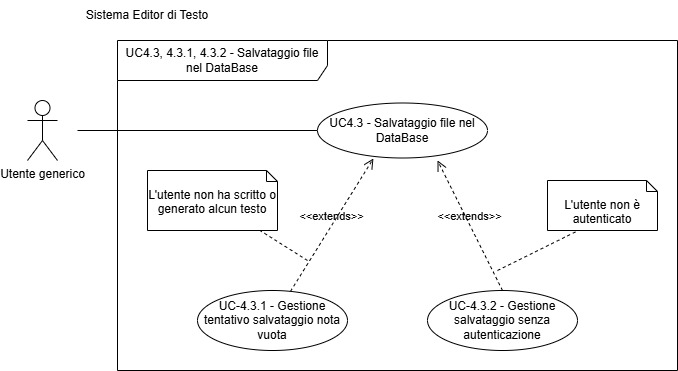
\includegraphics[width=0.8\textwidth]{../UCimg/UC4.3.jpg}
    \caption{Diagramma dei casi d'uso UC-4.3, 4.3.1, 4.3.2}
    \label{fig:uc4.3}
\end{figure}

\newpage

\subsection{Macroarea 5 - Autenticazione}
\subsubsection{UC-5.0 - Login}
\begin{itemize}
    \item \textbf{Attore principale}: \gls{Utente non autenticato}
    \item \textbf{Descrizione}: Permette all'utente di accedere al proprio account, rendendo così disponibili funzionalità di salvataggio, modifica e cancellazione di documenti nel db, salvati a nome dell'utente
    \item \textbf{Precondizioni}: L'utente è già registrato presso il sistema
    \item \textbf{Postcondizioni}: All'utente è permesso accedere al suo account nel sistema
    \item \textbf{Scenario principale}:
        \begin{itemize}
            \item L'utente accede al sistema
            \item L'utente seleziona la funzionalità Login
            \item L'utente inserisce un username ed una password univoci nel sistema
            \item All'utente viene permesso l'accesso
        \end{itemize}
    \item \textbf{Estensioni}:
        \begin{itemize}
            \item L'utente inserisce un username non presente nel db
            \item L'utente inserisce un username esistente ma la password sbagliata
        \end{itemize}
\end{itemize}

\subsubsection{UC-5.0.1 - Gestione username inesistente}
\begin{itemize}
    \item \textbf{Attore principale}: \gls{Utente non autenticato}
    \item \textbf{Descrizione}: Il sistema gestisce il tentativo di accesso con un identificativo utente non presente nel \gls{database}
    \item \textbf{Precondizioni}: L’utente ha inviato una richiesta di login
    \item \textbf{Postcondizioni}: L’accesso viene negato e viene mostrato un messaggio di errore generico
    \item \textbf{Scenario principale}:
    \begin{itemize}
        \item Il sistema interroga il \gls{database} alla ricerca dell'username fornito
        \item Il sistema non rileva alcuna corrispondenza (account inesistente)
        \item Il sistema nega l'accesso
        \item Il sistema mostra all’utente un messaggio di avviso generico
        \item L'utente rimane nella schermata di login
    \end{itemize}
\end{itemize}

\subsubsection{UC-5.0.2 - Gestione password errata}
\begin{itemize}
    \item \textbf{Attore principale}: \gls{Utente non autenticato}
    \item \textbf{Descrizione}: Il sistema gestisce il tentativo di accesso con un username valido ma associato a una password non corrispondente
    \item \textbf{Precondizioni}: L’utente ha inviato una richiesta di login con un username esistente
    \item \textbf{Postcondizioni}: L’accesso viene negato e viene mostrato un messaggio di errore generico
    \item \textbf{Scenario principale}:
    \begin{itemize}
        \item Il sistema rileva che l'username esiste
        \item Il sistema \gls{verifica} la corrispondenza crittografica della password inserita con quella memorizzata
        \item Il sistema rileva una incongruenza
        \item Il sistema nega l'accesso
        \item Il sistema mostra all’utente un messaggio di avviso generico
        \item L'utente rimane nella schermata di login
    \end{itemize}
\end{itemize}

\subsubsection{UC-5.1 - Registrazione}
\begin{itemize}
    \item \textbf{Attore principale}: \gls{Utente non autenticato}
    \item \textbf{Descrizione}: L'utente potrà creare un nuovo account nel sistema accedendo così alle funzionalità di salvataggio, modifica e cancellazione di documenti nel db, salvati a nome dell'utente
    \item \textbf{Precondizioni}: L'utente non è ancora autenticato nel sistema
    \item \textbf{Postcondizioni}: L'utente possiede un account nel sistema individuato da un username ed una password
    \item \textbf{Scenario principale}:
        \begin{itemize}
            \item L'utente accede al sistema
            \item L'utente seleziona la funzionalità "Registrati"
            \item L'utente inserisce un username univoco nel sistema
            \item L'utente inserisce una password che rispetta i vincoli
        \end{itemize}
    \item \textbf{Estensioni}:
        \begin{itemize}
            \item L'utente inserisce un username già esistente nel sistema
        \end{itemize}
\end{itemize}

\subsubsection{UC-5.1.1 - Gestione username già esistente}
\begin{itemize}
\item \textbf{Attore principale}: \gls{Utente non autenticato}
\item \textbf{Descrizione}: Il sistema impedisce la creazione di un account duplicato se l'identificativo scelto è già presente nel \gls{database}
\item \textbf{Precondizioni}: L’utente ha inviato i dati per la registrazione
\item \textbf{Postcondizioni}: La registrazione viene bloccata e l'utente viene avvisato
\item \textbf{Scenario principale}:
\begin{itemize}
\item Il sistema controlla la disponibilità dell'username (o email) nel \gls{database}
\item Il sistema rileva che l'username è già associato a un account esistente
\item Il sistema blocca la creazione del nuovo record
\item Il sistema visualizza un messaggio di errore
\item L'utente viene riportato al modulo di login
\end{itemize}
\end{itemize}

\begin{figure}[H]
    \centering
    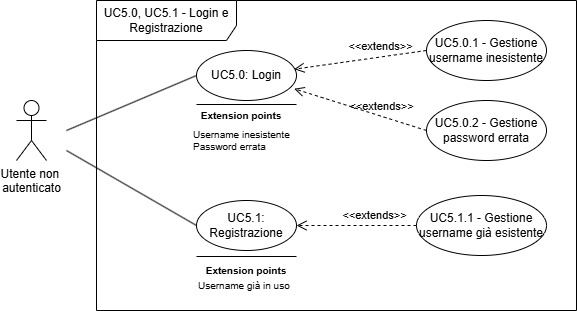
\includegraphics[width=0.8\textwidth]{../UCimg/UC5.0.jpg}
    \caption{Diagramma dei casi d'uso UC-5.0, 5.0.*, 5.1, 5.1.*}
    \label{fig:uc5.0}
\end{figure}


\subsubsection{UC-5.2 - Eliminazione dell'account}
\begin{itemize}
    \item \textbf{Attore principale}: \gls{Utente autenticato}
    \item \textbf{Descrizione}: L'utente decide di eliminare il proprio account dal sistema
    \item \textbf{Precondizioni}: L'utente è autenticato nel sistema
    \item \textbf{Postcondizioni}: L'account dell'utente viene eliminato dal sistema e l'utente non potrà più accedere alle funzionalità relative alle sue note
    \item \textbf{Scenario principale}:
        \begin{itemize}
            \item L'utente accede al sistema
            \item L'utente seleziona l'opzione "Elimina account"
            \item Il sistema mostra un pop up di conferma della scelta
            \item L'utente accetta e viene sloggato
            \item Il sistema elimina dal db il nome utente e la password relative all'attore
        \end{itemize}
    \item \textbf{Estensioni}:
        \begin{itemize}
            \item L'utente seleziona "annulla" nel pop up di conferma
        \end{itemize}
\end{itemize}

\subsubsection{UC-5.2.1 - Annullamento della procedura di eliminazione account}
\begin{itemize}
    \item \textbf{Attore principale}: \gls{Utente autenticato}
    \item \textbf{Descrizione}: Il sistema gestisce l'interruzione della procedura di eliminazione su richiesta dell'utente
    \item \textbf{Precondizioni}: È visualizzata la richiesta di conferma per l'eliminazione dell'account
    \item \textbf{Postcondizioni}: La procedura viene interrotta, l'account rimane attivo e i dati intatti
    \item \textbf{Scenario principale}:
    \begin{itemize}
        \item L’utente, di fronte alla richiesta di conferma, seleziona l’opzione ”Annulla” (o chiude il popup)
        \item Il sistema chiude la finestra di dialogo
        \item Il sistema abortisce l'operazione di cancellazione sul \gls{database}
        \item L'utente viene riportato alla schermata delle impostazioni del profilo nello stato precedente
    \end{itemize}
\end{itemize}

\begin{figure}[H]
    \centering
    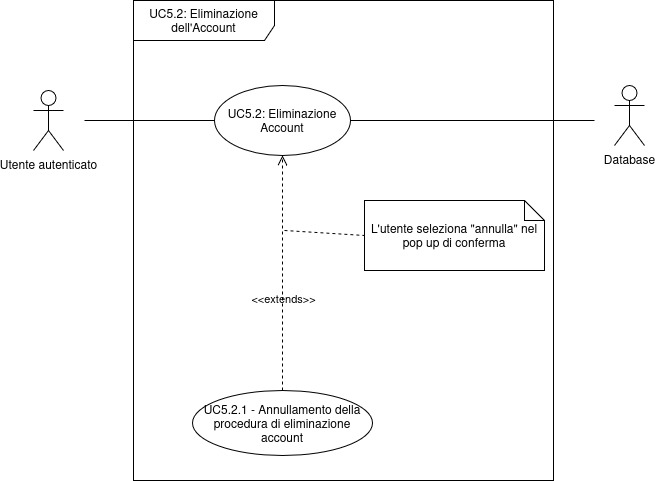
\includegraphics[width=0.8\textwidth]{../UCimg/UC5.2.jpg}
    \caption{Diagramma dei casi d'uso UC-5.2, 5.2.1}
    \label{fig:uc5.2}
\end{figure}


\subsubsection{UC-5.3 - Logout}
\begin{itemize}
    \item \textbf{Attore principale}: \gls{Utente autenticato}
    \item \textbf{Descrizione}: L'utente desidera terminare la propria sessione
    \item \textbf{Precondizioni}: L'utente è autenticato nel sistema
    \item \textbf{Postcondizioni}: L'utente viene disconnesso dal sistema
    \item \textbf{Scenario principale}:
        \begin{itemize}
            \item L'utente accede al sistema
            \item L'utente desidera disconnettersi
            \item L'utente seleziona l'opzione "Logout"
            \item L'utente viene disconnesso dal sistema
            \item La sessione dell'utente termina
            \item L'utente viene riportato alla pagina iniziale
        \end{itemize}
\end{itemize}

\begin{figure}[H]
    \centering
    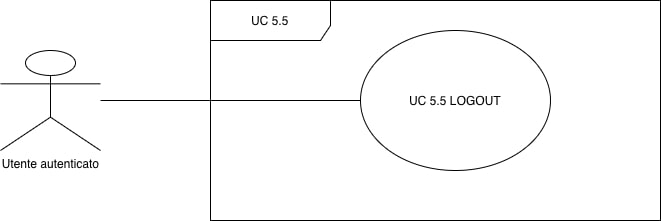
\includegraphics[width=0.8\textwidth]{../UCimg/UC5.3.jpg}
    \caption{Diagramma del caso d'uso UC-5.3}
    \label{fig:uc5.3}
\end{figure}

\newpage

\section{Requisiti}
\subsection{Classificazione dei requisiti}
Il gruppo ByteMe durante l'\gls{analisi dei requisiti} e dei casi d'uso ha individuato i requisiti esposti di seguito.
I requisiti sono stati classificati secondo una notazione standardizzata per garantirne la tracciabilità e una chiara comprensione.
Ogni requisito è identificato da un codice univoco che ne esplicita l'importanza e la tipologia.

\subsubsection{Notazione standardizzata dei requisiti}
Il codice identificativo segue il formato:
\[
R[Importanza]-[Tipo]-[Numero]
\]
Dove le voci assumono i seguenti significati:

\begin{description}
    \item[Importanza] \hfill \\
    Indica il grado di priorità del requisito:
    \begin{itemize}
        \item \textbf{O (Obbligatorio):} Requisito esplicitamente richiesto dall'azienda Zucchetti. La sua mancata implementazione implica il fallimento degli obiettivi primari del progetto.
        \item \textbf{D (Desiderabile):} Requisito non strettamente vincolante ma che il gruppo si impegna ad implementare per migliorare il prodotto.
        \item \textbf{OP (Opzionale):} Requisito di priorità minore, la cui implementazione può essere rimandata.
    \end{itemize}
    
    \item[Tipo] \hfill \\
    Indica la natura del requisito:
    \begin{itemize}
        \item \textbf{F (Funzionale):} Descrive le funzionalità e i servizi che il sistema deve fornire.
        \item \textbf{V (Vincolo):} Descrive limitazioni tecnologiche, normative o implementative imposte esternamente.
        \item \textbf{Q (Qualità):} Descrive le caratteristiche qualitative del sistema (es. performance, sicurezza, manutenibilità).
    \end{itemize}
    
    \item[Numero] \hfill \\
    Un numero intero progressivo univoco per tipologia di requisito.
\end{description}

\subsection{Categorie dei requisiti}
Per una maggiore chiarezza espositiva, i requisiti sono stati suddivisi in tre macro-categorie distinte.

\subsubsection{\gls{Requisiti funzionali}}
I \gls{requisiti funzionali} definiscono i comportamenti specifici del sistema, descrivendo le interazioni tra gli attori e il software.
Rappresentano le funzionalità tangibili che l'utente utilizza per raggiungere i propri obiettivi (es. scrittura del testo, selezione per analisi AI, esportazione documenti). La \gls{verifica} di tali requisiti determina l'aderenza del prodotto alle funzioni richieste dal capitolato.

\begin{longtable}{|p{0.2\textwidth}|>{\raggedright\arraybackslash}p{0.5\textwidth}|p{0.2\textwidth}|}
\hline
\textbf{Requisito} & \textbf{Descrizione} & \textbf{Casi d'uso correlati}\\
\hline
\endhead
% OBBLIGATORI
RO-F-1 & Il sistema deve fornire un'area di testo per l'inserimento e la modifica del testo con supporto alla sintassi \gls{Markdown} standard (CommonMark). & UC-1.0 \\
\hline
RO-F-2 & Il sistema deve informare l'utente con un messaggio in caso di perdita della connessione Internet durante l'utilizzo dell'editor. & UC-1.0.1 \\
\hline
RO-F-3 & Il sistema deve informare l'utente con un messaggio se l'editor non risponde ai comandi. & UC-1.0.2 \\
\hline
RO-F-4 & L'editor deve compilare la sintassi \gls{Markdown} in tempo reale. & UC-1.1 \\
\hline
RO-F-5 & Deve essere presente un'area di visualizzazione del documento formattato rispetto alla sintassi \gls{Markdown}. & UC-1.1 \\
\hline
RO-F-6 & Il sistema deve informare l'utente con un messaggio se il pannello di anteprima non si aggiorna correttamente. & UC-1.1.1 \\
\hline
RO-F-7 & Il sistema deve permettere all'utente di selezionare porzioni di testo tramite mouse o tastiera. & UC-1.2, UC-2.6, UC-2.7, UC-2.7.*, UC-2.9, UC-2.10 \\
\hline
RO-F-8 & Il sistema deve permettere all'utente di modificare porzioni di testo selezionate. & UC-1.2 \\
\hline
RO-F-9 & Il sistema deve permettere all'utente di copiare una parte di testo selezionato. & UC-1.3 \\
\hline
RO-F-10 & Il sistema deve permettere all'utente di incollare un testo nell'area di testo. & UC-1.4 \\
\hline
RO-F-11 & Il sistema deve permettere all'utente di tagliare il testo selezionato. & UC-1.5 \\
\hline
RO-F-12 & Il sistema deve permettere all'utente di annullare l'ultima modifica effettuata. & UC-1.6 \\
\hline
RO-F-13 & Se non sono presenti operazioni annullabili, il sistema non esegue alcuna azione al comando Undo. & UC-1.6.1 \\
\hline
RO-F-14 & Il sistema deve permettere all'utente di ripristinare le modifiche precedentemente annullate. & UC-1.7 \\
\hline
RO-F-15 & Se non sono presenti operazioni ripristinabili, il sistema non esegue alcuna azione al comando Redo. & UC-1.7.1 \\
\hline
RO-F-16 & Nell'editor deve essere presente una barra degli strumenti (\gls{toolbar}) per applicare formattazioni \gls{Markdown} senza scrivere manualmente la sintassi. & UC-1.8.0, UC-1.8.* \\
\hline
RO-F-17 & Il sistema deve permettere l'applicazione del grassetto al testo tramite \gls{toolbar}. & UC-1.8.2 \\
\hline
RO-F-18 & Il sistema deve permettere l'applicazione del corsivo al testo tramite \gls{toolbar}. & UC-1.8.3 \\
\hline
RO-F-19 & Il sistema deve permettere l'applicazione della sottolineatura al testo tramite \gls{toolbar}. & UC-1.8.4 \\
\hline
RO-F-20 & Il sistema deve permettere di creare intestazioni tramite \gls{toolbar}. & UC-1.8.5 \\
\hline
RO-F-21 & Il sistema deve permettere l'inserimento di elementi di struttura (tabelle, separatori orizzontali) tramite \gls{toolbar}. & UC-1.8.6 \\
\hline
RO-F-22 & Il sistema deve permettere l'inserimento di liste numerate tramite \gls{toolbar}. & UC-1.8.7 \\
\hline
RO-F-23 & Il sistema deve permettere l'inserimento di elenchi puntati tramite \gls{toolbar}. & UC-1.8.7 \\
\hline
RO-F-24 & Il sistema deve permettere l'inserimento di link e riferimenti tramite \gls{toolbar}. & UC-1.8.8 \\
\hline
RO-F-25 & L'utente può applicare più stili contemporaneamente (es. grassetto, corsivo, sottolineatura) alla stessa sezione di testo. & UC-1.8.* \\
\hline
RO-F-26 & L'utente può annullare una formattazione di una porzione di testo selezionato riapplicandola dalla \gls{toolbar}. & UC-1.8.1 \\
\hline
RO-F-27 & L'utente può estendere la formattazione a una porzione di testo parzialmente formattato riapplicandola dalla \gls{toolbar}. & UC-1.8.0.1 \\
\hline
RO-F-28 & L'utente può creare sottoliste attivando la creazione di una lista dalla \gls{toolbar} quando il cursore è già all'interno di una lista. & UC-1.8.7.1 \\
\hline
RO-F-29 & L'utente può scegliere una combinazione di formattazioni dalla \gls{toolbar} quando non è presente testo selezionato, per applicarle al testo che scriverà successivamente. & UC-1.9.* \\
\hline
RO-F-30 & Il sistema deve permettere all'utente di selezionare porzioni di testo da inviare all'agente esterno. & UC-1.2, UC-2.* \\
\hline
RO-F-31 & Il sistema permette di inviare del testo ad un agente esterno. & UC-2.* \\
\hline
RO-F-32 & L'utente deve poter accedere alle azioni sul testo tramite agente esterno in ogni momento. & UC-2.* \\
\hline
RO-F-33 & Il testo generato viene prima mostrato come proposta, separata visivamente dal testo dell'utente. & UC-2.1 \\
\hline
RO-F-34 & Il testo in stato di proposta include le opzioni di conferma, annullamento e rigenerazione. & UC-2.1 \\
\hline
RO-F-35 & Il sistema non permette la modifica del testo generato mentre è in stato di proposta. & UC-2.* \\
\hline
RO-F-36 & Il testo generato dall'agente esterno, una volta confermato, viene inserito nella posizione del cursore se presente, altrimenti in fondo al testo. & UC-2.1.1 \\
\hline
RO-F-37 & Una proposta che viene confermata viene inserita nel documento nell'editor e la sezione di proposta viene rimossa. & UC-2.1.1 \\
\hline
RO-F-38 & Una volta generato e confermato, il testo dell'agente esterno è modificabile tramite le stesse funzionalità dell'editor disponibili per il testo utente. & UC-2.1.1 \\
\hline
RO-F-39 & Una proposta annullata comporta la rimozione del testo generato dalla sezione di proposta e la rimozione della sezione stessa. & UC-2.1.2 \\
\hline
RO-F-40 & Una proposta che viene rigenerata viene rimandata all'agente esterno con gli stessi parametri e la nuova risposta sovrascrive la proposta corrente. & UC-2.1.3 \\
\hline
RO-F-41 & Il sistema deve informare l'utente con un messaggio in caso di errore durante la comunicazione con il servizio LLM. & UC-2.1.4 \\
\hline
RO-F-42 & L'utente può annullare un'operazione AI in corso prima del suo completamento. & UC-2.1.5 \\
\hline
RO-F-43 & In seguito all'annullamento di un'operazione AI, il documento rimane nello stato precedente alla richiesta. & UC-2.1.5 \\
\hline
RO-F-44 & Se la generazione di testo si blocca prematuramente, rimane ciò che è già stato generato, in attesa che l'utente confermi, rigeneri o elimini la proposta. & UC-2.* \\
\hline
RO-F-45 & L'agente esterno applica modifiche esclusivamente al testo selezionato dall'utente. Un contesto aggiuntivo può essere fornito solo a scopo interpretativo e non deve essere alterato. & UC-2.* \\
\hline
RO-F-46 & L'utente può consultare il registro delle generazioni AI effettuate. & UC-2.0 \\
\hline
RO-F-47 & Il sistema deve gestire il caso in cui lo storico delle generazioni AI sia vuoto, informando l'utente con un messaggio appropriato. & UC-2.0.1 \\
\hline
RO-F-48 & Ogni generazione di testo dell'agente esterno viene inclusa nel registro delle generazioni, incluse quelle annullate dall'utente. & UC-2.0, UC-2.1 \\
\hline
RO-F-49 & Il sistema deve permettere all'utente di visualizzare il testo completo di una generazione dallo storico AI. & UC-2.0.3 \\
\hline
RO-F-50 & L'utente deve poter riassumere tutto o una parte selezionata del testo usando un agente esterno. & UC-2.2 \\
\hline
RO-F-51 & L'utente deve poter usare un agente esterno per riscrivere tutto o una parte selezionata del testo migliorandolo seguendo determinate specifiche come sintassi, stile e chiarezza. & UC-2.3 \\
\hline
RO-F-52 & L'utente deve poter tradurre il testo usando un agente esterno in: inglese, italiano, tedesco, francese, spagnolo e cinese mandarino. & UC-2.4.* \\
\hline
RO-F-53 & Se l'utente avvia una traduzione senza selezionare la lingua di destinazione, il sistema lo notifica e blocca l'operazione. & UC-2.4.1 \\
\hline
RO-F-54 & Il sistema permette di avviare la correzione grammaticale del testo tramite agente esterno. & UC-2.5 \\
\hline
RO-F-55 & Se non vengono rilevati errori grammaticali, il sistema informa l'utente dell'esito positivo della correzione. & UC-2.5.1 \\
\hline
RO-F-56 & Il sistema consente all'utente di avviare l'analisi critica del testo selezionato o dell'intero documento utilizzando il cappello di De Bono scelto. & UC-2.6 \\
\hline
RO-F-57 & Se il testo è insufficiente per l'analisi critica, il sistema notifica l'utente e interrompe l'operazione. & UC-2.6.1 \\
\hline
RO-F-58 & Se l'utente avvia l'analisi critica senza selezionare un cappello di De Bono, il sistema lo notifica e blocca l'operazione. & UC-2.6.2 \\
\hline
RO-F-59 & Il sistema permette l'invio di un \gls{prompt} scritto dall'utente per la generazione di testo tramite agente esterno. & UC-2.7 \\
\hline
RO-F-60 & Il sistema permette la modifica del \gls{prompt} da inviare all'agente esterno prima dell'invio. & UC-2.7 \\
\hline
RO-F-61 & L'agente esterno può generare testo basandosi su un \gls{prompt} fornitogli dall'utente. & UC-2.7.* \\
\hline
RO-F-62 & Se il \gls{prompt} fornito dall'utente è vuoto o incompleto, il sistema notifica l'utente e impedisce l'invio. & UC-2.7.1 \\
\hline
RO-F-63 & L'utente può caricare un file dal proprio dispositivo all'interno dell'editor. & UC-3.* \\
\hline
RO-F-64 & Il sistema deve supportare il caricamento di file in formato \gls{Markdown} (\texttt{.md}, \texttt{.\gls{markdown}}) e testo semplice (\texttt{.txt}). & UC-3.0, UC-3.0.1, UC-3.0.2 \\
\hline
RO-F-65 & Il sistema deve supportare il caricamento tramite dialogo di esplorazione file (file picker). & UC-3.0.4 \\
\hline
RO-F-66 & Prima di procedere con il caricamento di un file, il sistema chiede conferma all'utente. & UC-3.0 \\
\hline
RO-F-67 & Il sistema deve informare l'utente con un messaggio di esito (successo o errore) al termine di ogni tentativo di caricamento file. & UC-3.1, UC-3.2 \\
\hline
RO-F-68 & Il sistema deve validare il formato del file selezionato e impedire il caricamento di formati non supportati. & UC-3.1 \\
\hline
RO-F-69 & Il sistema deve validare le dimensioni del file selezionato e impedire il caricamento di file che superano la dimensione massima consentita. & UC-3.2 \\
\hline
RO-F-70 & Il sistema deve impedire il caricamento di file corrotti o illeggibili. & UC-3.1 \\
\hline
RO-F-71 & Il sistema deve permettere all'utente di rimuovere il file che ha caricato. & UC-3.3 \\
\hline
RO-F-72 & L'utente può annullare l'operazione di rimozione del file caricato, lasciando l'editor nel suo stato precedente. & UC-3.3.1 \\
\hline
RO-F-73 & Il sistema deve essere in grado di convertire il documento da \gls{Markdown} al formato selezionato dall'utente. & UC-4.0 \\
\hline
RO-F-74 & Il sistema deve permettere di scaricare il file nel dispositivo dell'utente. & UC-4.0 \\
\hline
RO-F-75 & L'operazione di esportazione o stampa non deve alterare né chiudere il documento originale nell'editor. & UC-4.* \\
\hline
RO-F-76 & Il sistema deve informare l'utente con un messaggio di esito al termine di ogni operazione di esportazione. & UC-4.0 \\
\hline
RO-F-77 & Il sistema deve consentire l'esportazione del documento in formato \gls{Markdown} (\texttt{.md}). & UC-4.0.2 \\
\hline
RO-F-78 & Il sistema deve controllare che il range di pagine inserito dall'utente sia valido (non superiore al numero di pagine del documento e non negativo). & UC-4.0.6, UC-4.0.7 \\
\hline
RO-F-79 & Il sistema deve permettere di collegare e inviare il documento a un dispositivo di stampa. & UC-4.1 \\
\hline
RO-F-80 & Il sistema deve informare l'utente con un messaggio in caso di errore durante l'invio del documento alla stampante. & UC-4.1 \\
\hline

% DESIDERABILI
RD-F-1 & Il sistema deve supportare l'uso di scorciatoie da tastiera per le operazioni di formattazione & UC-1.3 - UC-1.8.* \\
\hline
RD-F-2 & Il sistema deve permettere di cambiare modalità di visualizzazione (Solo Editor, Solo Anteprima, Split View) & UC-1.10.* \\
\hline
RD-F-3 & Il sistema deve supportare il caricamento tramite drag-and-drop (trascinamento file nell'area dell'editor) & UC-3.0.3 \\
\hline
RD-F-4 & Se sono presenti modifiche non salvate nell'editor, il sistema chiede conferma all'utente prima di caricare un nuovo file, permettendo di annullare l'operazione, per salvare il testo presente, o sovrascrivere il contenuto senza salvarlo & UC-3.0 \\
\hline
RD-F-5 & Il parsing del contenuto del file caricato deve gestire caratteri non validi senza causare il crash dell'applicazione. & UC-3.0.* \\
\hline
RD-F-6 & I messaggi di errore relativi al caricamento file (formato non supportato, file troppo grande, file corrotto) devono essere esplicativi e suggerire come procedere. & UC-3.1, UC-3.2 \\
\hline
RD-F-7 & Il sistema deve offrire più opzioni per le operazioni comuni sui file come carica nuovo, stampa, chiudi & UC-3.0, UC-3.3, UC-4.0, UC-4.1\\
\hline
RD-F-8 & Il sistema deve consentire l'esportazione del documento in formato PDF & UC-4.0.1 \\
\hline
RD-F-9 & Il sistema deve consentire l'esportazione del documento in formato HTML & UC-4.0.3 \\
\hline
RD-F-10 & Il sistema deve consentire l'esportazione del documento in formato ODT & UC-4.0.4 \\
\hline
RD-F-11 & Il sistema deve consentire l'esportazione del documento in formato DOCX & UC-4.0.5 \\
\hline
RD-F-12 & L'utente deve poter scegliere se esportare l'intero documento o un range di pagine selezionate & UC-4.0.6, UC-4.0.7\\
\hline
RD-F-13 & Il sistema deve consentire all'utente di scegliere il nome del file prima di procedere al download/esportazione. & UC-4.0 \\
\hline
RD-F-14 & Il sistema deve fornire un'anteprima del documento nel formato selezionato prima di procedere al download. & UC-4.0 \\
\hline
RD-F-15 & Il sistema deve aprire il dialogo di stampa nativo del browser, tramite il quale l'utente può configurare le opzioni di stampa disponibili (inclusa la selezione delle pagine). & UC-4.1 \\
\hline

% OPZIONALI
ROP-F-1 & L'utente può ricercare parole nel testo attraverso l'editor & UC-1.11 \\
\hline
ROP-F-2 & Il sistema deve informare l'utente se la ricerca non ha prodotto occorrenze nel testo. & UC-1.11.1 \\
\hline
ROP-F-3 & La sezione di testo generata come proposta è visibilmente diversa dal testo utente & UC-2.* \\
\hline
ROP-F-4 & Per ogni voce del registro delle generazioni AI il sistema deve indicare la data e l'ora della generazione. & UC-2.0.2 \\
\hline
ROP-F-5 & Per ogni voce del registro delle generazioni AI il sistema deve indicare il tipo di operazione che ha prodotto la generazione. & UC-2.0.2 \\
\hline
ROP-F-6 & L'utente può eliminare una voce dal registro delle generazioni AI. & UC-2.0.4 \\
\hline
ROP-F-7 & Per gli utenti autenticati, il registro delle generazioni AI è persistente ed è associato ai documenti salvati nel proprio account. & UC-2.0.5 \\
\hline
ROP-F-8 & La sezione di testo in stato di proposta viene colorata in base al tipo di operazione che viene fatta & UC-2.1 \\
\hline
ROP-F-9 & Il sistema deve visualizzare sia il testo originale che la traduzione generata, permettendo all'utente di confrontarle. & UC-2.4.* \\
\hline
ROP-F-10 & Se il testo selezionato è già nella lingua di destinazione della traduzione, il sistema avvisa l'utente e interrompe l'operazione. & UC-2.4.* \\
\hline
ROP-F-11 & Il sistema offre esempi per la richiesta di generazione di testo a partire da un estratto & UC-2.7 \\
\hline
ROP-F-12 & Il sistema permette di inserire un grafico generato, con dati presenti nel testo, scelto tra diversi tipi disponibili all'utente & UC-2.8 \\
\hline
ROP-F-13 & Il sistema permette di inserire una tabella generata con dati presenti nel testo & UC-2.8 \\
\hline
ROP-F-14 & Se i dati nel testo sono insufficienti per generare grafici o tabelle, il sistema notifica l'utente. & UC-2.8.1 \\
\hline
ROP-F-15 & Il sistema permette di inserire una mappa concettuale generata con dati presenti nel testo & UC-2.9 \\
\hline
ROP-F-16 & Se si verificano errori nella visualizzazione della mappa concettuale generata, il sistema notifica l'utente. & UC-2.9.1 \\
\hline
ROP-F-17 & Il sistema permette di inserire una formula matematica generata con dati presenti nel testo & UC-2.10 \\
\hline
ROP-F-18 & Se la formula matematica contiene simboli non supportati, il sistema notifica l'utente. & UC-2.10.1 \\
\hline
ROP-F-19 & Il sistema deve permettere all'utente di inserire le proprie credenziali (username e password) per il login & UC-5.0 \\
\hline
ROP-F-20 & Se le credenziali sono errate il sistema non permette all'utente di autenticarsi & UC-5.0.* \\
\hline
ROP-F-21 & Il sistema deve mostrare un messaggio di errore generico in caso di fallimento del login, senza specificare se l'errore riguarda username o password. & UC-5.0.1, UC-5.0.2 \\
\hline
ROP-F-22 & In caso di username già esistente durante la registrazione, il sistema deve proporre all'utente di effettuare il login o scegliere un nuovo username. & UC-5.1.1 \\
\hline
ROP-F-23 & Il sistema deve permettere all'utente di potersi registrare tramite uno username e una password & UC-5.1 \\
\hline
ROP-F-24 & Il sistema deve impedire la registrazione in caso ci sia uno username uguale nel \gls{database} & UC-5.1 \\
\hline
ROP-F-25 & Il sistema deve salvare nel \gls{database} le password criptate in fase di registrazione & UC-5.1 \\
\hline
ROP-F-26 & Il sistema deve permettere ad un \gls{utente autenticato} di poter eliminare il proprio account & UC-5.2 \\
\hline
ROP-F-27 & Il sistema in caso di eliminazione account deve eliminare i dati dal \gls{database} & UC-5.2 \\
\hline
ROP-F-28 & Le operazioni di eliminazione dell'account devono richiedere una conferma esplicita da parte dell'utente & UC-5.2 \\
\hline
ROP-F-29 & Il sistema deve terminare la sessione se un account viene eliminato & UC-5.2 \\
\hline
ROP-F-30 & L'utente può annullare la procedura di eliminazione del proprio account. & UC-5.2.1 \\
\hline
ROP-F-31 & Il sistema deve permettere ad un utente di vedere i file che ha salvato & UC-4.2 \\
\hline
ROP-F-32 & Il sistema deve permettere ad un \gls{utente autenticato} di selezionare un file dall'elenco di quelli salvati e aprirlo & UC-4.2 \\
\hline
ROP-F-33 & Il sistema deve permettere all'utente di annullare l'operazione di apertura file, lasciando l'editor nel suo stato precedente. & UC-4.2.1 \\
\hline
ROP-F-34 & Il sistema deve mostrare i file salvati in ordine cronologico per data di ultima modifica. & UC-4.2 \\
\hline
ROP-F-35 & L'accesso ai file salvati nel \gls{database} è consentito solo ad utenti autenticati. & UC-4.2 \\
\hline
ROP-F-36 & Il sistema deve permettere il salvataggio di un file in un \gls{sistema di persistenza} non locale & UC-4.3 \\
\hline
ROP-F-37 & Il sistema deve notificare l'utente in caso di fallimento del salvataggio nel \gls{database}. & UC-4.3 \\
\hline
ROP-F-38 & Il sistema deve associare ogni file al suo creatore & UC-4.3 \\
\hline
ROP-F-39 & Il sistema deve impedire il salvataggio di file nel \gls{database} da parte di utenti non autenticati. & UC-4.3, UC-4.3.2 \\
\hline
ROP-F-40 & Il sistema deve impedire il salvataggio di un documento vuoto nel \gls{database}. & UC-4.3.1 \\
\hline
ROP-F-41 & Un \gls{utente non autenticato} che prova a salvare un file viene riportato alla pagina di login & UC-4.3.2 \\
\hline
ROP-F-42 & L'utente può effettuare il logout in ogni momento e terminare la propria sessione & UC-5.3 \\
\hline
\addlinespace[1em]
\caption{Tabella dei \gls{requisiti funzionali}}
\end{longtable}

\newpage
\subsubsection{\gls{Requisiti di vincolo}}
I \gls{requisiti di vincolo} rappresentano le limitazioni entro le quali il progetto deve essere sviluppato. A differenza dei \gls{requisiti funzionali}, questi non derivano da scelte progettuali del team, ma sono imposizioni esterne dettate dal committente, da normative o da limiti tecnologici. Questi comprendono i vincoli tecnologici, architetturali e organizzativi.

\begin{longtable}{|p{0.15\textwidth}|>{
  \raggedright\arraybackslash}p{0.55\textwidth}|p{0.2\textwidth}|}
\hline
\textbf{Requisito} & \textbf{Descrizione} & \textbf{Fonte} \\
\hline
RO-V-1 & L'applicazione deve essere accessibile tramite browser web. 
I browser supportati sono: Google Chrome ($\geq$ v110), Mozilla Firefox 
($\geq$ v110), Microsoft Edge ($\geq$ v110), Safari ($\geq$ v16). & Capitolato \\
\hline
RO-V-2 & Il sistema deve utilizzare la codifica Unicode (UTF-8) per la rappresentazione interna e lo storage del testo. & Capitolato \\
\hline
RO-V-3 & Il formato di input e di storage del testo deve essere \gls{Markdown}, in conformità allo standard CommonMark. & Capitolato \\
\hline
RO-V-4 & Il sistema deve integrarsi con un servizio LLM tramite \gls{API} REST compatibili con lo standard OpenAI. & Capitolato \\
\hline
\addlinespace[1em]
\caption{Tabella dei \gls{requisiti di vincolo}}
\end{longtable}

\newpage

\subsubsection{\gls{Requisiti di qualità}}
I \gls{requisiti di qualità} specificano le caratteristiche 
misurabili del software e della documentazione. Non descrivono nuove 
funzionalità, ma stabiliscono soglie quantitative che il sistema deve 
rispettare, verificabili tramite le metriche definite nel 
Piano di Qualifica v1.0.0.

\begin{longtable}{|p{0.15\textwidth}|>{\raggedright\arraybackslash}
  p{0.55\textwidth}|p{0.2\textwidth}|}
\hline
\textbf{Requisito} & \textbf{Descrizione} & \textbf{Fonte} \\
\hline
RO-Q-1 & Il tempo di risposta dell'interfaccia utente (aggiornamento anteprima, applicazione formattazioni) deve essere inferiore a 500 ms nel 95\% dei casi, misurato su una sessione utente attiva di almeno 30 minuti.  & PdQ – Response Time, soglia accettabile \\
\hline
RO-Q-2 & Il tempo medio di generazione di una risposta da parte del servizio LLM non deve superare i 10 secondi, misurato su un campione di almeno 20 richieste consecutive in condizioni di utilizzo normale.  & PdQ – AI Processing Time, soglia accettabile \\
\hline
RO-Q-3 & Il tasso di errori nelle operazioni principali (salvataggio, apertura file, chiamate AI) non deve superare l'1\%, misurato sul totale delle operazioni eseguite in una sessione utente attiva di almeno 30 minuti. & PdQ – Error Rate, soglia accettabile \\
\hline
RO-Q-4 & La percentuale di codice coperta dai test automatici (test coverage) deve essere almeno il 70\%, misurata sull'insieme completo dei moduli rilasciati ad ogni versione. & PdQ – Test Coverage, soglia accettabile \\
\hline
RO-Q-5 & La complessità ciclomatica (McCabe) di ogni funzione/metodo del codice prodotto non deve superare il valore 8. & PdQ – Complessità Ciclomatica, soglia accettabile \\
\hline
RO-Q-6 & La documentazione prodotta deve ottenere un Indice di Gulpease (IG) maggiore o uguale a 40. & PdQ – Indice di Gulpease, soglia accettabile \\
\hline
RO-Q-7 & Il sistema deve essere sviluppato rispettando le Norme 
di Progetto del gruppo ByteMe. & \gls{Norme di Progetto} v1.0.0 \\
\hline
RO-Q-8 & Il sistema deve essere verificato secondo il Piano di Qualifica prima di ogni rilascio. & Piano di Qualifica v1.0.0 \\
\hline
RO-Q-9 & Il \gls{manuale utente} deve documentare tutte le funzionalità obbligatorie del sistema e deve ottenere un Indice di Gulpease (IG) maggiore o uguale a 40. & PdQ – Indice di Gulpease, soglia accettabile \\
\hline
RO-Q-10 & Il manuale di installazione e deployment del sistema deve ottenere un Indice di Gulpease (IG) maggiore o uguale a 40. & PdQ – Indice di Gulpease, soglia accettabile \\
\hline
\addlinespace[1em]
\caption{Tabella dei \gls{requisiti di qualità}}
\end{longtable}

\newpage

\subsection{Tracciamento}
\subsubsection{Fonte - Requisiti}
\begin{longtable}{|p{0.2\textwidth}|p{0.45\textwidth}|>{\raggedright\arraybackslash}p{0.25\textwidth}|}
\hline
\textbf{Caso d'uso} & \textbf{Descrizione} & \textbf{Requisiti} \\
\hline
\endhead
UC-1.0 & Scrittura nell'editor & RO-F-1 \\
\hline
UC-1.0.1 & Gestione perdita connessione Internet & RO-F-2 \\
\hline
UC-1.0.2 & Gestione errore di risposta dell'editor & RO-F-3 \\
\hline
UC-1.1 & Visualizzazione anteprima in tempo reale & RO-F-4, RO-F-5 \\
\hline
UC-1.1.1 & Gestione errore nell'anteprima & RO-F-6 \\
\hline
UC-1.2 & Selezione del testo & RO-F-7, RO-F-8, RO-F-30 \\
\hline
UC-1.3 & Copiare il testo & RO-F-9 \\
\hline
UC-1.4 & Incollare il testo & RO-F-10 \\
\hline
UC-1.5 & Tagliare il testo & RO-F-11 \\
\hline
UC-1.6 & Annullamento modifica (Undo) & RO-F-12 \\
\hline
UC-1.6.1 & Gestione assenza di modifiche annullabili & RO-F-13 \\
\hline
UC-1.7 & Ripristino modifica (Redo) & RO-F-14 \\
\hline
UC-1.7.1 & Errore per modifiche non ripristinabili & RO-F-15 \\
\hline
UC-1.8.0 & Modifica testo selezionato tramite \gls{toolbar} & RO-F-16 \\
\hline
UC-1.8.0.1 & Testo già parzialmente formattato & RO-F-27 \\
\hline
UC-1.8.1 & Rimozione formattazione tramite \gls{toolbar} & RO-F-26 \\
\hline
UC-1.8.2 & Applicazione grassetto & RO-F-17 \\
\hline
UC-1.8.3 & Applicazione corsivo & RO-F-18 \\
\hline
UC-1.8.4 & Applicazione sottolineatura & RO-F-19 \\
\hline
UC-1.8.5 & Applicazione intestazioni & RO-F-20 \\
\hline
UC-1.8.6 & Inserimento elementi di struttura & RO-F-21 \\
\hline
UC-1.8.7 & Inserimento liste ed elenchi & RO-F-22, RO-F-23, RO-F-25 \\
\hline
UC-1.8.7.1 & Gestione sotto-liste & RO-F-28 \\
\hline
UC-1.8.8 & Inserimento link e riferimenti & RO-F-24 \\
\hline
UC-1.9 & Impostare formattazioni senza testo & RO-F-29 \\
\hline
UC-1.9.1 & Impostare grassetto al testo futuro & RO-F-29 \\
\hline
UC-1.9.2 & Impostare corsivo al testo futuro & RO-F-29 \\
\hline
UC-1.9.3 & Impostare sottolineatura al testo futuro & RO-F-29 \\
\hline
UC-1.9.4 & Impostare intestazioni & RO-F-29 \\
\hline
UC-1.9.5 & Impostare struttura al documento & RO-F-29 \\
\hline
UC-1.9.6 & Impostare liste ed elenchi & RO-F-29 \\
\hline
UC-1.9.7 & Impostare link e riferimenti & RO-F-29 \\
\hline
UC-1.10 & Gestione modalità di visualizzazione & RD-F-2 \\
\hline
UC-1.10.1 & Modalità solo editor & RD-F-2 \\
\hline
UC-1.10.2 & Modalità solo documento formattato & RD-F-2 \\
\hline
UC-1.10.3 & Modalità split view & RD-F-2 \\
\hline
UC-1.11 & Ricerca nel testo & ROP-F-1 \\
\hline
UC-1.11.1 & Gestione assenza di occorrenze & ROP-F-2 \\
\hline
UC-2.0 & Visualizzazione storico generazioni AI & RO-F-46, RO-F-48 \\
\hline
UC-2.0.1 & Visualizzazione storico generazioni vuoto & RO-F-47 \\
\hline
UC-2.0.2 & Visualizzazione titolo generazione & ROP-F-4, ROP-F-5 \\
\hline
UC-2.0.3 & Visualizzazione testo generato & RO-F-49 \\
\hline
UC-2.0.4 & Eliminazione generazione dallo storico & ROP-F-6 \\
\hline
UC-2.0.5 & Storico generazioni per utente registrato & ROP-F-7 \\
\hline
UC-2.1 & Interazione con testi generati dall'AI & RO-F-33, RO-F-34, RO-F-35, RO-F-48, ROP-F-3, ROP-F-8 \\
\hline
UC-2.1.1 & Conferma testo generato & RO-F-36, RO-F-37, RO-F-38 \\
\hline
UC-2.1.2 & Eliminazione testo generato & RO-F-39 \\
\hline
UC-2.1.3 & Rigenerazione testo generato & RO-F-40 \\
\hline
UC-2.1.4 & Errore dal LLM & RO-F-41 \\
\hline
UC-2.1.5 & Annullamento operazione AI & RO-F-42, RO-F-43 \\
\hline
UC-2.2 & Riassunto del testo & RO-F-50 \\
\hline
UC-2.3 & Riscrittura del testo & RO-F-51 \\
\hline
UC-2.4 & Traduzione del testo & RO-F-52, ROP-F-9 \\
\hline
UC-2.4.1 & Gestione mancata selezione lingua & RO-F-53 \\
\hline
UC-2.4.2 & Traduzione in inglese & RO-F-52 \\
\hline
UC-2.4.3 & Traduzione in spagnolo & RO-F-52 \\
\hline
UC-2.4.4 & Traduzione in francese & RO-F-52 \\
\hline
UC-2.4.5 & Traduzione in tedesco & RO-F-52 \\
\hline
UC-2.4.6 & Traduzione in cinese mandarino & RO-F-52 \\
\hline
UC-2.4.7 & Traduzione in italiano & RO-F-52, ROP-F-10 \\
\hline
UC-2.5 & Correzione grammaticale & RO-F-54 \\
\hline
UC-2.5.1 & Nessun errore grammaticale rilevato & RO-F-55 \\
\hline
UC-2.6 & Critica testuale con i 6 Cappelli di De Bono & RO-F-56 \\
\hline
UC-2.6.1 & Gestione testo insufficiente per analisi & RO-F-57 \\
\hline
UC-2.6.2 & Gestione mancata selezione modalità analisi & RO-F-58 \\
\hline
UC-2.6.3 & Critica con Cappello Bianco & RO-F-56 \\
\hline
UC-2.6.4 & Critica con Cappello Rosso & RO-F-56 \\
\hline
UC-2.6.5 & Critica con Cappello Nero & RO-F-56 \\
\hline
UC-2.6.6 & Critica con Cappello Giallo & RO-F-56 \\
\hline
UC-2.6.7 & Critica con Cappello Verde & RO-F-56 \\
\hline
UC-2.6.8 & Critica con Cappello Blu & RO-F-56 \\
\hline
UC-2.7 & Generazione di testo (\gls{Distant Writing}) & RO-F-59, RO-F-60, RO-F-61, ROP-F-11 \\
\hline
UC-2.7.1 & Gestione \gls{prompt} incompleto & RO-F-62 \\
\hline
UC-2.8 & Generazione di grafici e tabelle & ROP-F-12, ROP-F-13 \\
\hline
UC-2.8.1 & Dati insufficienti per grafici e tabelle & ROP-F-14 \\
\hline
UC-2.9 & Generazione di mappe concettuali & ROP-F-15 \\
\hline
UC-2.9.1 & Errori visualizzazione mappe concettuali & ROP-F-16 \\
\hline
UC-2.10 & Generazione di formule matematiche & ROP-F-17 \\
\hline
UC-2.10.1 & Gestione simboli non supportati & ROP-F-18 \\
\hline
UC-3.0 & Caricamento file & RO-F-63, RO-F-64, RO-F-66, RD-F-4, RD-F-7 \\
\hline
UC-3.0.1 & Caricamento file \gls{Markdown} & RO-F-64 \\
\hline
UC-3.0.2 & Caricamento file di testo & RO-F-64 \\
\hline
UC-3.0.3 & Opzione trascina file & RD-F-3 \\
\hline
UC-3.0.4 & Opzione esplora file & RO-F-65 \\
\hline
UC-3.1 & Gestione formati file non supportati & RO-F-67, RO-F-68, RO-F-70, RD-F-6 \\
\hline
UC-3.2 & Gestione file troppo grandi & RO-F-67, RO-F-69, RD-F-6 \\
\hline
UC-3.3 & Rimozione file caricato & RO-F-71, RD-F-7 \\
\hline
UC-3.3.1 & Annullamento rimozione file & RO-F-72 \\
\hline
UC-4.0 & Esportazione di un file & RO-F-73, RO-F-74, RO-F-76, RD-F-7, RD-F-13, RD-F-14 \\
\hline
UC-4.0.1 & Esportazione in PDF & RD-F-8 \\
\hline
UC-4.0.2 & Esportazione in MD & RO-F-77 \\
\hline
UC-4.0.3 & Esportazione in HTML & RD-F-9 \\
\hline
UC-4.0.4 & Esportazione in ODT & RD-F-10 \\
\hline
UC-4.0.5 & Esportazione in DOCX & RD-F-11 \\
\hline
UC-4.0.6 & Esportazione pagine selezionate & RO-F-78, RD-F-12 \\
\hline
UC-4.0.7 & Esportazione range di pagine & RO-F-78, RD-F-12 \\
\hline
UC-4.1 & Stampare il documento & RO-F-75, RO-F-79, RO-F-80, RD-F-7, RD-F-15 \\
\hline
UC-4.2 & Apertura di un file salvato & ROP-F-31, ROP-F-32, ROP-F-34, ROP-F-35 \\
\hline
UC-4.2.1 & Gestione annullamento apertura & ROP-F-33 \\
\hline
UC-4.3 & Salvataggio file nel \gls{database} & ROP-F-36, ROP-F-37, ROP-F-38, ROP-F-39 \\
\hline
UC-4.3.1 & Gestione salvataggio nota vuota & ROP-F-40 \\
\hline
UC-4.3.2 & Gestione salvataggio senza autenticazione & ROP-F-39, ROP-F-41 \\
\hline
UC-5.0 & Login & ROP-F-19 \\
\hline
UC-5.0.1 & Gestione username inesistente & ROP-F-20, ROP-F-21 \\
\hline
UC-5.0.2 & Gestione password errata & ROP-F-20, ROP-F-21 \\
\hline
UC-5.1 & Registrazione & ROP-F-23, ROP-F-24, ROP-F-25 \\
\hline
UC-5.1.1 & Gestione username già esistente & ROP-F-22 \\
\hline
UC-5.2 & Eliminazione dell'account & ROP-F-26, ROP-F-27, ROP-F-28, ROP-F-29 \\
\hline
UC-5.2.1 & Annullamento eliminazione account & ROP-F-30 \\
\hline
UC-5.3 & Logout & ROP-F-42 \\
\hline
\addlinespace[1em]
\caption{Tracciamento casi d'uso - \gls{requisiti funzionali}}
\end{longtable}

\newpage

\section{Riepilogo}
\begin{table}[H]
\centering
\begin{tabular}{|p{0.2\textwidth}|>{\raggedright\arraybackslash}p{0.1\textwidth}|p{0.1\textwidth}|p{0.1\textwidth}|p{0.1\textwidth}|}
\hline
\textbf{Tipologia} & \textbf{O} & \textbf{D} & \textbf{OP} & \textbf{Totale}\\
\hline
Funzionali & 80 & 15 & 42 & 137 \\
\hline
Vincolo & 4 & 0 & 0 & 4 \\
\hline
Qualità & 10 & 0 & 0 & 10 \\
\hline
\textbf{Totale} & 94 & 15 & 42 & 151 \\
\hline
\end{tabular}
\caption{Riepilogo dei requisiti}
\end{table}

\end{document}
